\documentclass[11pt]{article}

\usepackage[margin=1.2in]{geometry}
\usepackage{amsmath,amssymb}
\usepackage[T1]{fontenc}
\usepackage[utf8]{inputenc}
\usepackage{lmodern}
\usepackage{microtype}
\usepackage{booktabs}
\usepackage[hidelinks,hypertexnames=false]{hyperref}
\usepackage{parskip}
\usepackage{enumitem}
\PassOptionsToPackage{dvipsnames}{xcolor}
\usepackage{tikz}
\usepackage{xcolor}
\usetikzlibrary{positioning, shapes.geometric, decorations.pathmorphing, arrows.meta, calc, patterns}
\usepackage{tcolorbox}
\newtcolorbox{keymessage}{%
  colback=blue!3, colframe=blue!40!black,
  fonttitle=\bfseries\small, title=Key Message,
  boxrule=0.5pt, arc=2pt, left=6pt, right=6pt, top=4pt, bottom=4pt
}

\title{The Map and the Territory:\\
A Constructive History of Mathematical Physics}
\author{Paul Chun-Kit Lee\\[2pt]
\small New York University\\[2pt]
\small\texttt{dr.paul.c.lee@gmail.com}}
\date{February 2026}

\begin{document}
\maketitle

\begin{abstract}
This essay tells the story of 150~years of mathematical physics from an unfamiliar angle.
A machine-verified research programme---approximately 25,400~lines of formally checked proofs in the Lean~4 proof assistant---provides preliminary evidence that for every exactly solvable model and system with explicit finite-size bounds examined so far, empirical predictions of quantum mechanics, statistical mechanics, general relativity, and classical mechanics can be derived using only the most elementary constructive logic, without the law of excluded middle or any principle of omniscience.
Paper~29 \cite{Lee2026paper29Fekete} establishes a fundamental qualification: Fekete's Subadditive Lemma---the generic tool for thermodynamic-limit convergence---is equivalent to LPO over BISH, making the logical cost ineliminable for systems near phase transitions where no explicit bounds exist.
The elaborate classical superstructure of modern physics---infinite-dimensional Hilbert spaces, thermodynamic limits, path integrals, singularity theorems---enters only through idealizations that no finite laboratory can instantiate.
The resulting hierarchy of logical strength is a partial order, not a chain: three independent branches (Dependent Choice, Markov's Principle, and the omniscience spine BISH~$<$~LLPO~$<$~WLPO~$<$~LPO) meet at the Fan Theorem in a fourth direction, with a refined choice hierarchy (CC~$<$~DC) separating ensemble from individual convergence along a second axis (Paper~25), and the logical cost of each idealization depends on the observable being computed, not merely the physical system under study.
This essay traces how classical logic was progressively imported into mathematical physics from the 1870s onward, what it cost at each stage, what constructive alternatives existed or could have been used instead, and what the pattern implies for the current state of theoretical physics.
This is Paper~12 in the Constructive Calibration Programme, a companion to the formal synthesis (Paper~10) \cite{Lee2026paper10}, written for a broader audience.
The calibration covers quantum states, static structures, and exactly solvable models; time evolution, scattering amplitudes, and real-time path integrals remain uncalibrated.
    The human-AI collaborative methodology is described in Appendix~\ref{app:collaboration}.
    These results are preliminary; we expect that experts in the constructive mathematics and Lean communities will identify errors and sharpen or correct the calibrations presented here.
\end{abstract}

% ============================================================
\section{The Cellar and the Cathedral}
% ============================================================

The most precise prediction in the history of science is a number: the anomalous magnetic moment of the electron, usually called $g{-}2$.
Quantum electrodynamics predicts this quantity to roughly twelve decimal places, and experiment confirms it.
The agreement is so exact that if you measured the distance from New York to Los Angeles to the same relative precision, you would be accurate to the width of a human hair.

Here is the quiet scandal behind that triumph.
Every step of the actual computation is finite arithmetic.
A physicist draws a Feynman diagram---a small picture of particles interacting---and translates it into a definite integral over a finite number of momentum variables.
She evaluates the integral numerically, adds contributions from a finite number of diagrams at each level of approximation, and arrives at a rational number with controlled error bars.
Every operation could be performed by a mechanical calculator given enough time.
There is no step that requires surveying an infinite set, deciding an undecidable question, or asserting the existence of a completed infinite object.

And yet the formalism in which this computation is embedded is a cathedral of infinities.
The path integral---the foundational tool of quantum field theory---is, in its continuum formulation, an ``integral'' over an infinite-dimensional space of field configurations for which no mathematically rigorous measure exists in general.
(Euclidean lattice path integrals---Wilson's 1974 construction \cite{Wilson1974}---are mathematically rigorous but operate on finite lattices, i.e., at BISH.)
Fock space, the mathematical arena for multi-particle quantum mechanics, is an infinite-dimensional tensor product.
Renormalization, the procedure that extracts finite predictions from divergent expressions, involves manipulations with quantities that are formally infinite.
The vacuum state---the ``empty'' starting point of every calculation---is a vector in an infinite-dimensional space whose properties encode the entire structure of the theory.

\begin{figure}[ht]
\centering
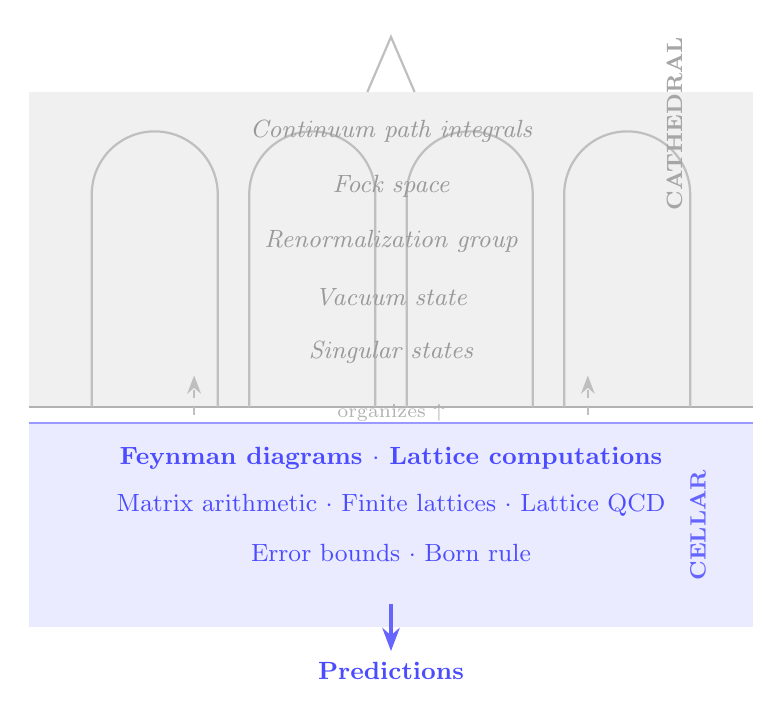
\begin{tikzpicture}[
  >=Stealth,
  every node/.style={font=\small}
]
% Cathedral (upper level) — shaded gray
\fill[gray!12] (-4.6, 2.8) rectangle (4.6, 6.8);
\draw[thick, gray!60] (-4.6, 2.8) -- (4.6, 2.8);
% Arches
\foreach \x in {-3, -1, 1, 3} {
  \draw[gray!50, thick] (\x-0.8, 2.8) -- (\x-0.8, 5.5) arc (180:0:0.8) -- (\x+0.8, 2.8);
}
% Spire
\draw[gray!50, thick] (-0.3, 6.8) -- (0, 7.5) -- (0.3, 6.8);
% Cathedral labels
\node[font=\small\itshape, gray!80] at (0, 6.3) {Continuum path integrals};
\node[font=\small\itshape, gray!80] at (0, 5.6) {Fock space};
\node[font=\small\itshape, gray!80] at (0, 4.9) {Renormalization group};
\node[font=\small\itshape, gray!80] at (0, 4.2) {Vacuum state};
\node[font=\small\itshape, gray!80] at (0, 3.5) {Singular states};
\node[font=\footnotesize\bfseries, gray!70] at (3.6, 6.4) {\rotatebox{90}{CATHEDRAL}};

% Cellar (lower level) — shaded blue
\fill[blue!8] (-4.6, 0) rectangle (4.6, 2.6);
\draw[thick, blue!40] (-4.6, 2.6) -- (4.6, 2.6);
% Cellar labels
\node[font=\small\bfseries, blue!70] at (0, 2.15) {Feynman diagrams $\cdot$ Lattice computations};
\node[font=\small, blue!70] at (0, 1.55) {Matrix arithmetic $\cdot$ Finite lattices $\cdot$ Lattice QCD};
\node[font=\small, blue!70] at (0, 0.95) {Error bounds $\cdot$ Born rule};
\node[font=\footnotesize\bfseries, blue!60] at (3.9, 1.3) {\rotatebox{90}{CELLAR}};

% Arrow: predictions flow up
\draw[->, very thick, blue!60] (0, 0.3) -- (0, -0.3) node[below, font=\small\bfseries, blue!70] {Predictions};

% Arrow: formalism sits above
\draw[->, thick, gray!50, dashed] (-2.5, 2.7) -- (-2.5, 3.2);
\draw[->, thick, gray!50, dashed] (2.5, 2.7) -- (2.5, 3.2);
\node[font=\scriptsize, gray!60] at (0, 2.73) {organizes $\uparrow$};

\end{tikzpicture}
\caption{The cellar and the cathedral. Every empirical prediction of quantum field theory examined so far (below) is a finite computation---BISH\@. The infinite-dimensional formalism (above) organizes the computations but is not itself physically instantiated. For tier~3 systems (generic phase transitions), Paper~29 shows the cathedral is not merely organizational but ineliminable (Section~\ref{sec:thesis}).}
\label{fig:cellar-cathedral}
\end{figure}

The predictions come from the cellar.
The cathedral sits above: beautiful, architecturally magnificent, and largely empty.
Almost nobody computes a continuum path integral; in perturbative QFT, they compute Feynman diagrams, and in lattice QCD, they evaluate discretized path integrals on finite lattices---both BISH operations.
Nobody works in Fock space; they work with definite, finite numbers of particles.
The infinite-dimensional superstructure is a mnemonic---a way of organizing the finite computations---but the physics, the part that touches experiment, lives in the finite arithmetic below (Figure~\ref{fig:cellar-cathedral}).

This essay is about the gap between the cellar and the cathedral.
It is about the question: how much of the mathematical apparatus of physics describes the physical world, and how much describes the mathematician's toolkit?
For the first time, a machine-verified research programme can answer this question with mathematical precision.
The answer is surprising, and it reaches back 150~years.
Every empirical prediction from a specific, tractable model that we have examined---across quantum mechanics, statistical mechanics, and general relativity---lives at the most elementary level of constructive logic.
For these systems, the classical superstructure, with its completed infinities and its implicit appeals to omniscience over infinite sets, is the mapmaker's convention.
Nature, it appears, speaks a simpler language---most of the time.

A word of framing before we proceed.
The map is not useless---it is an extraordinarily effective organizing tool.
Classical mathematics has powered the greatest quantitative achievements in the history of science.
But the map is not always the territory.
The thesis of this essay is not that the classical formalism is wrong, but that for specific tractable models it contains more structure than the physics requires, and that the excess structure has gradually been mistaken for reality.
Paper~29 \cite{Lee2026paper29Fekete} reveals, however, that the story is richer: for generic systems near phase transitions, Fekete's Subadditive Lemma ($\equiv$ LPO) is the only mathematical route, and the mapmaker's convention becomes the territory itself (Section~\ref{sec:thesis}).
The constructive hierarchy provides a precise tool for separating the territory from the mapmaker's conventions---and for identifying where the conventions are ineliminable.

\begin{keymessage}
Every empirical prediction of QFT from specific tractable models examined in this programme is finite arithmetic --- constructive analysis at BISH\@.
The infinite-dimensional formalism organizes computations but is not physically instantiated for tiers~1--2.
The predictions come from the cellar; for these tiers, the cathedral is the mathematician's convenience.
For tier~3 (generic systems near criticality), Paper~29 shows the cathedral is ineliminable.
\end{keymessage}

A scope note: the calibration programme examines quantum states, static structures, and specific exactly solvable models---not quantum dynamics.
Time evolution, scattering amplitudes, the S-matrix, and real-time path integrals remain uncalibrated.
``BISH'' throughout this essay means Bishop-style constructive analysis---which includes real-valued computation with explicit moduli of convergence, not merely discrete or finite arithmetic.
The claims about empirical predictions should be read with both limitations in mind.


% ============================================================
\section{What Physicists Don't Know They're Assuming}
% ============================================================

To understand what the research programme has discovered, you need to understand a distinction that most physicists have never encountered: the difference between levels of \emph{logical strength} in mathematics.

Before describing the hierarchy, a crucial clarification.
The hierarchy of logical strength (BISH $<$ WLPO $<$ LPO $<$ LEM) measures what \emph{principles} a proof requires---what kind of assertions about infinite sets you must accept.
This is entirely different from Turing undecidability, which measures what no \emph{algorithm} can compute regardless of the axioms you accept.
A problem can be Turing-decidable yet require LPO to prove (the thermodynamic limit), or Turing-undecidable yet live outside the omniscience hierarchy entirely (the spectral gap problem of Cubitt et~al.\ \cite{Cubitt2015}, which is Turing-undecidable).
The spectral gap is undecidable in the sense that no algorithm can determine the answer from a Hamiltonian's local rules; this is not ``a level above LEM'' in the logical hierarchy but an orthogonal phenomenon.
Throughout this essay, ``logical strength'' refers to the constructive hierarchy, not to computability in the Turing sense.

Consider an infinite hotel with rooms numbered 1, 2, 3, and so on.
You want to know whether every room is empty.
Here are four different things you might be allowed to assert, each representing a different level of logical power.

At the first level---call it \textbf{BISH}, for Bishop-style constructive mathematics \cite{Bishop1967}---you can check rooms one by one, and you can report what you find.
If you have a proof that works for every room (a master key, say, that shows no guest could possibly be registered), you may declare ``all empty.''
If you find an occupied room, you may point to it and say ``room 47 is occupied.''
But you may \emph{not} declare ``they're all empty'' without a universal proof, and you may not declare ``someone's home'' without producing the room number.
You claim only what you can demonstrate.

At the second level---\textbf{WLPO}, the Weak Limited Principle of Omniscience---you gain a modest superpower.
You may assert either ``all rooms are empty'' \emph{or} ``it is not the case that all rooms are empty.''
But in the second case, you do not need to produce the occupied room.
You know something is there; you just cannot point to it.

At the third level---\textbf{LPO}, the Limited Principle of Omniscience---you have full dichotomy.
Either ``all rooms are empty'' or ``here is the occupied room.''\footnote{Formally: for any binary sequence $\alpha : \mathbb{N} \to \{0,1\}$, either $\alpha(n) = 0$ for all $n$, or there exists $n$ with $\alpha(n) = 1$.}
No ambiguity, no gap between knowing something exists and finding it.

At the fourth level---\textbf{LEM}, the Law of Excluded Middle, which is the logic of standard mathematics---you can answer \emph{any} yes-or-no question about the hotel instantly.
Not just occupancy: any question whatsoever, about any collection of mathematical objects, has a definite true-or-false answer, whether or not you can determine which.

Between WLPO and LPO lie two further levels that the research programme has now populated with physical content.
At \textbf{LLPO}, the Lesser Limited Principle of Omniscience, you can determine the \emph{sign} of a nonzero quantity---``this is positive or this is negative''---without the full dichotomy of LPO\@.
In the hotel metaphor, you know the occupied rooms are all on even floors or all on odd floors, but you cannot point to a specific room.
LLPO is strictly between WLPO and LPO\@.
Separately, the \textbf{Fan Theorem} (FT) asserts that a pointwise property of all infinite paths through a finitely branching tree can be witnessed by a uniform finite bound.
FT is independent of the entire omniscience spine---it neither implies nor is implied by LPO---and occupies a distinct branch of the partial order.
In the hotel metaphor, FT says: if every guest checks out eventually, there is a uniform checkout time that works for all of them, without needing to know which room each guest occupied.

These levels form a partial order, not a simple chain: BISH is the weakest, LEM is the strongest, but there are independent branches (DC$_\omega$, MP, FT) that neither imply each other nor imply WLPO \cite{BridgesVita2006, BridgesRichman1987}.
The separations are strict---there are mathematical universes where WLPO holds but LPO fails, where LLPO holds but WLPO fails, and where FT holds but LPO fails.

The hierarchy is not esoteric.
Each step up the ladder is a specific claim about your ability to decide questions involving infinite collections.
BISH says: decide only what you can verify by a finite procedure.
LLPO says: you may determine the sign of a nonzero real.
WLPO says: you may know that something is true ``in principle'' without exhibiting a witness.
LPO says: you may decide existence claims about infinite sequences.
FT says: pointwise finiteness implies uniform finiteness.
LEM says: everything is decidable, period.

\begin{figure}[ht]
\centering
\resizebox{\textwidth}{!}{%
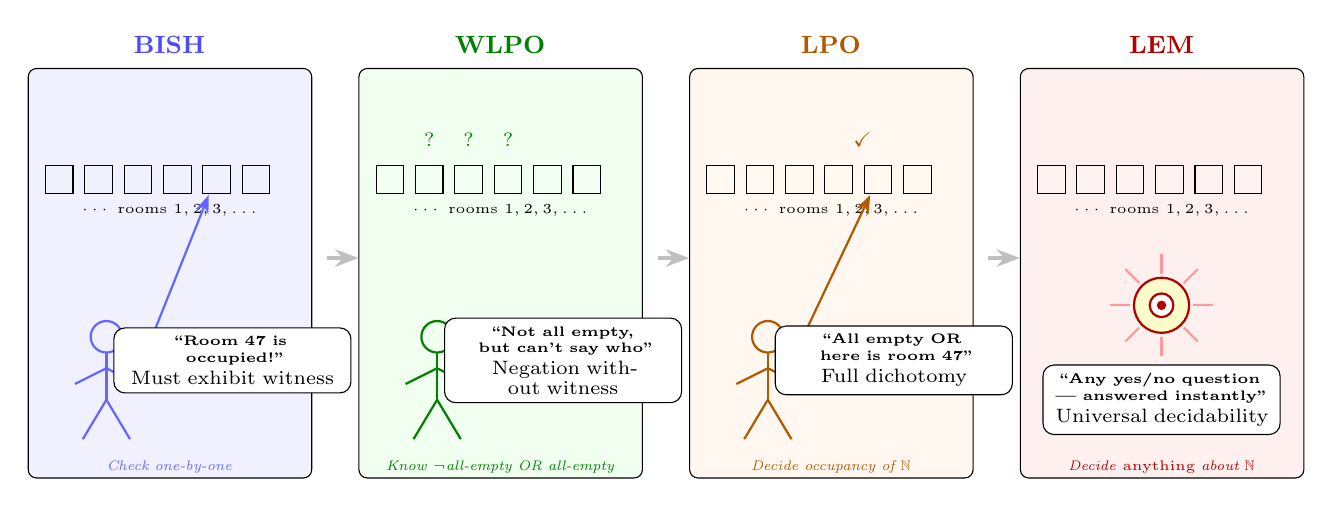
\begin{tikzpicture}[
  >=Stealth,
  panel/.style={draw, rounded corners=3pt, minimum width=3.6cm, minimum height=5.2cm, anchor=south west},
  roomstyle/.style={draw, minimum width=0.35cm, minimum height=0.35cm, inner sep=0pt},
  bubble/.style={draw, rounded corners=4pt, fill=white, font=\tiny, text width=2.8cm, align=center, inner sep=3pt}
]
% Panel 1: BISH
\node[panel, fill=blue!6] (p1) at (0,0) {};
\node[font=\small\bfseries, blue!70] at (1.8, 5.5) {BISH};
% Hotel rooms
\foreach \i in {0,...,5} {
  \node[roomstyle, fill=blue!5] at (0.4+\i*0.5, 3.8) {};
}
\node[font=\tiny] at (1.8, 3.4) {$\cdots$ rooms $1, 2, 3, \ldots$};
% Stick figure checking rooms
\draw[thick, blue!60] (1.0, 1.8) circle (0.2);
\draw[thick, blue!60] (1.0, 1.6) -- (1.0, 1.0);
\draw[thick, blue!60] (1.0, 1.4) -- (0.6, 1.2);
\draw[thick, blue!60] (1.0, 1.4) -- (1.4, 1.2);
\draw[thick, blue!60] (1.0, 1.0) -- (0.7, 0.5);
\draw[thick, blue!60] (1.0, 1.0) -- (1.3, 0.5);
% Arrow pointing to room
\draw[->, thick, blue!60] (1.5, 1.6) -- (2.3, 3.6);
% Speech bubble
\node[bubble] at (2.6, 1.5) {\textbf{``Room 47 is\\occupied!''}\\[2pt]\scriptsize Must exhibit witness};
\node[font=\tiny\itshape, blue!60] at (1.8, 0.15) {Check one-by-one};

% Panel 2: WLPO
\node[panel, fill=green!6] (p2) at (4.2,0) {};
\node[font=\small\bfseries, green!50!black] at (6.0, 5.5) {WLPO};
\foreach \i in {0,...,5} {
  \node[roomstyle, fill=green!5] at (4.6+\i*0.5, 3.8) {};
}
\node[font=\tiny] at (6.0, 3.4) {$\cdots$ rooms $1, 2, 3, \ldots$};
% Stick figure at desk
\draw[thick, green!50!black] (5.2, 1.8) circle (0.2);
\draw[thick, green!50!black] (5.2, 1.6) -- (5.2, 1.0);
\draw[thick, green!50!black] (5.2, 1.4) -- (4.8, 1.2);
\draw[thick, green!50!black] (5.2, 1.4) -- (5.6, 1.2);
\draw[thick, green!50!black] (5.2, 1.0) -- (4.9, 0.5);
\draw[thick, green!50!black] (5.2, 1.0) -- (5.5, 0.5);
% Question marks over rooms
\node[font=\scriptsize, green!50!black] at (5.1, 4.3) {?};
\node[font=\scriptsize, green!50!black] at (5.6, 4.3) {?};
\node[font=\scriptsize, green!50!black] at (6.1, 4.3) {?};
% Speech bubble
\node[bubble] at (6.8, 1.5) {\textbf{``Not all empty,\\but can't say who''}\\[2pt]\scriptsize Negation without witness};
\node[font=\tiny\itshape, green!50!black] at (6.0, 0.15) {Know $\lnot$all-empty OR all-empty};

% Panel 3: LPO
\node[panel, fill=orange!6] (p3) at (8.4,0) {};
\node[font=\small\bfseries, orange!70!black] at (10.2, 5.5) {LPO};
\foreach \i in {0,...,5} {
  \node[roomstyle, fill=orange!5] at (8.8+\i*0.5, 3.8) {};
}
\node[font=\tiny] at (10.2, 3.4) {$\cdots$ rooms $1, 2, 3, \ldots$};
% Oracle figure
\draw[thick, orange!70!black] (9.4, 1.8) circle (0.2);
\draw[thick, orange!70!black] (9.4, 1.6) -- (9.4, 1.0);
\draw[thick, orange!70!black] (9.4, 1.4) -- (9.0, 1.2);
\draw[thick, orange!70!black] (9.4, 1.4) -- (9.8, 1.2);
\draw[thick, orange!70!black] (9.4, 1.0) -- (9.1, 0.5);
\draw[thick, orange!70!black] (9.4, 1.0) -- (9.7, 0.5);
% Check mark and arrow
\draw[->, thick, orange!70!black] (9.8, 1.7) -- (10.7, 3.6);
\node[font=\scriptsize, orange!70!black] at (10.6, 4.3) {\checkmark};
% Speech bubble
\node[bubble] at (11.0, 1.5) {\textbf{``All empty OR\\here is room 47''}\\[2pt]\scriptsize Full dichotomy};
\node[font=\tiny\itshape, orange!70!black] at (10.2, 0.15) {Decide occupancy of $\mathbb{N}$};

% Panel 4: LEM
\node[panel, fill=red!6] (p4) at (12.6,0) {};
\node[font=\small\bfseries, red!70!black] at (14.4, 5.5) {LEM};
\foreach \i in {0,...,5} {
  \node[roomstyle, fill=red!5] at (13.0+\i*0.5, 3.8) {};
}
\node[font=\tiny] at (14.4, 3.4) {$\cdots$ rooms $1, 2, 3, \ldots$};
% God's eye
\draw[thick, red!70!black, fill=yellow!20] (14.4, 2.2) circle (0.35);
\draw[thick, red!70!black, fill=white] (14.4, 2.2) circle (0.15);
\fill[red!70!black] (14.4, 2.2) circle (0.06);
% Rays
\foreach \a in {0,45,...,315} {
  \draw[red!40, thick] (14.4, 2.2) ++ (\a:0.4) -- ++ (\a:0.25);
}
% Speech bubble
\node[bubble] at (14.4, 1.0) {\textbf{``Any yes/no question\\--- answered instantly''}\\[2pt]\scriptsize Universal decidability};
\node[font=\tiny\itshape, red!70!black] at (14.4, 0.15) {Decide \emph{anything} about $\mathbb{N}$};

% Arrows showing hierarchy
\draw[->, very thick, gray!50] (3.8, 2.8) -- (4.2, 2.8);
\draw[->, very thick, gray!50] (8.0, 2.8) -- (8.4, 2.8);
\draw[->, very thick, gray!50] (12.2, 2.8) -- (12.6, 2.8);

\end{tikzpicture}%
}% end resizebox
\caption{The infinite hotel at four logical levels.
\textbf{BISH}: you may assert only what you can verify by finite procedure.
\textbf{WLPO}: you may assert ``not all empty'' without producing the occupied room.
\textbf{LPO}: full dichotomy on infinite sequences---either all empty or exhibit a witness.
\textbf{LEM}: every yes/no question about any mathematical object has a definite answer.
Each level implies all those to its left; the implications are strict.}
\label{fig:hotel}
\end{figure}

Physicists work at the top of this ladder without a second thought.
Every proof in a standard textbook uses the law of excluded middle freely: a particle is either in this region or it isn't; a sequence either converges or it doesn't; a geodesic either terminates or it extends forever.
The question this essay addresses is whether the physics \emph{needs} all that logical power, or whether the predictions would survive with less.

Think of it this way.
Every theorem in a physics textbook has an invisible footnote reading: ``This proof also assumes that you can survey infinite sets in a single glance.''
The research programme described here identifies which theorems genuinely need that footnote and which would stand without it.

\begin{figure}[ht]
\centering
\resizebox{\textwidth}{!}{%
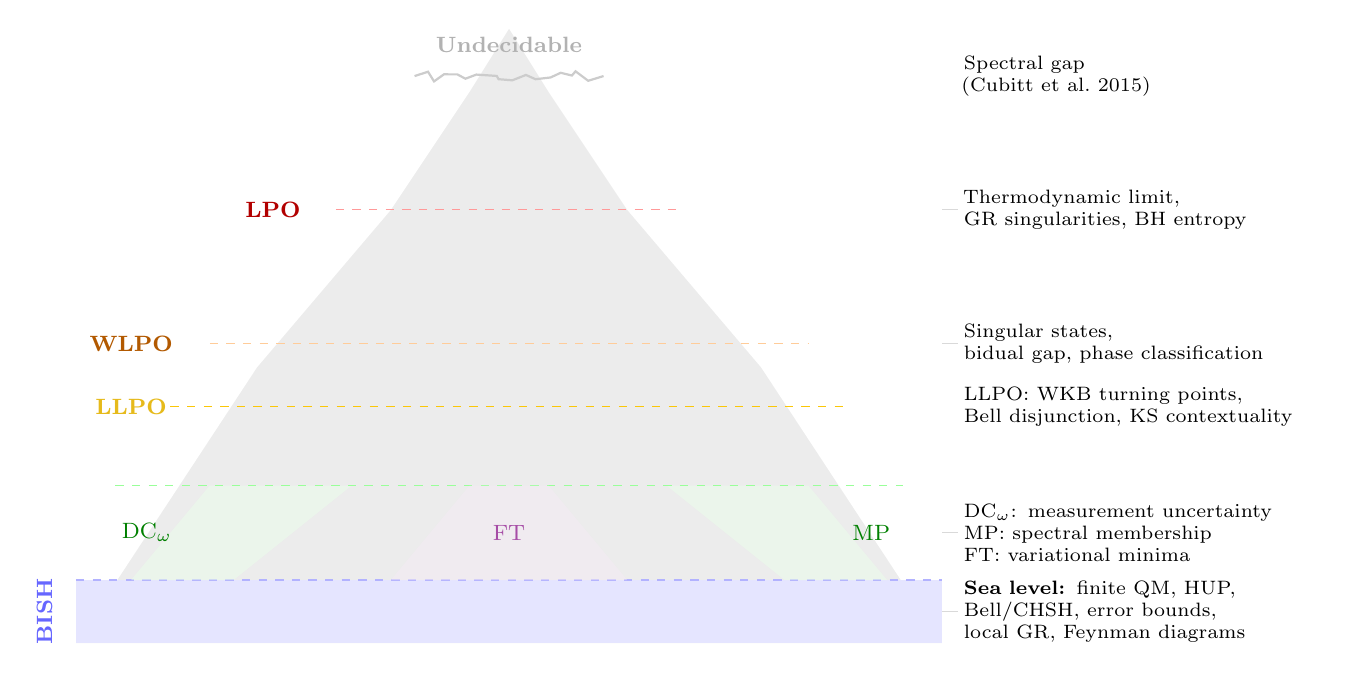
\begin{tikzpicture}[
  >=Stealth,
  every node/.style={font=\small},
  physlabel/.style={font=\scriptsize, text width=4.5cm, align=left, inner sep=2pt}
]
% Mountain body
\fill[gray!15] (-5.5,0) -- (-3.2, 3.5) -- (-1.5, 5.5) -- (-0.5, 7.0) -- (0, 7.8) -- (0.5, 7.0) -- (1.5, 5.5) -- (3.2, 3.5) -- (5.5, 0) -- cycle;
% Altitude bands — shaded
\fill[blue!10] (-5.5, 0) -- (-5.5, 0.8) -- (5.5, 0.8) -- (5.5, 0) -- cycle;
\draw[blue!30, dashed] (-5.5, 0.8) -- (5.5, 0.8);
% Sea level label
\node[font=\footnotesize\bfseries, blue!60] at (-5.9, 0.4) {\rotatebox{90}{BISH}};
% Foothills
\fill[green!8, opacity=0.5] (-4.8, 0.8) -- (-3.8, 2.0) -- (-2.0, 2.0) -- (-3.5, 0.8) -- cycle;
\fill[green!8, opacity=0.5] (3.5, 0.8) -- (2.0, 2.0) -- (3.8, 2.0) -- (4.8, 0.8) -- cycle;
\draw[green!40, dashed] (-5.0, 2.0) -- (5.0, 2.0);
\node[font=\footnotesize, green!50!black] at (-4.6, 1.4) {\footnotesize DC$_\omega$};
\node[font=\footnotesize, green!50!black] at (4.6, 1.4) {\footnotesize MP};
% LLPO ledge — raised to avoid foothills label overlap
\draw[yellow!60!orange, dashed] (-4.3, 3.0) -- (4.3, 3.0);
\node[font=\footnotesize\bfseries, yellow!60!orange!90!black] at (-4.8, 3.0) {LLPO};
% FT foothill (independent branch)
\fill[violet!8, opacity=0.5] (-1.5, 0.8) -- (-0.5, 2.0) -- (0.5, 2.0) -- (1.5, 0.8) -- cycle;
\node[font=\footnotesize, violet!70] at (0, 1.4) {\footnotesize FT};
% Mountainside — raised to keep gap from LLPO
\draw[orange!40, dashed] (-3.8, 3.8) -- (3.8, 3.8);
\node[font=\footnotesize\bfseries, orange!70!black] at (-4.8, 3.8) {WLPO};
% Summit
\draw[red!40, dashed] (-2.2, 5.5) -- (2.2, 5.5);
\node[font=\footnotesize\bfseries, red!70!black] at (-3.0, 5.5) {LPO};
% Cloud at top
\draw[gray!40, thick, decorate, decoration={random steps, segment length=4pt, amplitude=2pt}]
  (-1.2, 7.2) -- (1.2, 7.2);
\node[font=\footnotesize\bfseries, gray!60] at (0, 7.6) {Undecidable};

% Physics labels on right
\node[physlabel, anchor=west] at (5.7, 0.4)
  {\textbf{Sea level:} finite QM, HUP,\\Bell/CHSH, error bounds,\\local GR, Feynman diagrams};
\node[physlabel, anchor=west] at (5.7, 1.4)
  {DC$_\omega$: measurement uncertainty\\MP: spectral membership\\FT: variational minima};
\node[physlabel, anchor=west] at (5.7, 3.0)
  {LLPO: WKB turning points,\\Bell disjunction, KS contextuality};
\node[physlabel, anchor=west] at (5.7, 3.8)
  {Singular states,\\bidual gap, phase classification};
\node[physlabel, anchor=west] at (5.7, 5.5)
  {Thermodynamic limit,\\GR singularities, BH entropy};
\node[physlabel, anchor=west] at (5.7, 7.2)
  {Spectral gap\\(Cubitt et al.\ 2015)};

% Connecting lines
\foreach \y/\xr in {0.4/5.5, 1.4/5.5, 3.8/5.5, 5.5/5.5} {
  \draw[gray!30, thin] (5.5, \y) -- (\xr+0.2, \y);
}

\end{tikzpicture}%
}% end resizebox
\caption{The logical geography of mathematical physics, depicted as a mountain.
Sea level (BISH) contains all empirical predictions from specific, tractable models (tiers~1--2). Higher altitudes correspond to
greater logical strength---stronger principles, not greater computational complexity. The summit (LPO) is ineliminable for generic systems near criticality (tier~3; Paper~29).
DC$_\omega$, MP, and FT occupy independent foothills---none implies any other, and none
implies WLPO\@.
LLPO occupies a ledge between the foothills and the mountainside.
The summit (LPO) contains the thermodynamic limit, singularity theorems, and BH entropy convergence.
Beyond it lies Turing undecidability, which is orthogonal to the logical-strength hierarchy.}
\label{fig:mountain}
\end{figure}

To give the hierarchy a visual anchor, imagine a mountain (Figure~\ref{fig:mountain}).
Sea level is BISH---constructive mathematics, finite procedures, the logic of computation.
The foothills are occupied by Dependent Choice, Markov's Principle, and the Fan Theorem---modest extensions that allow countable sequences of choices, conclude existence from the impossibility of non-existence, or extract uniform bounds from pointwise data.
These three foothills are \emph{independent}: none implies any other, and none implies WLPO.
The mountain has ridges running in different directions.
A ledge at LLPO---the Lesser Limited Principle of Omniscience---sits between the foothills and the mountainside.
LLPO governs sign decisions: it lets you determine whether a nonzero quantity is positive or negative without the full witness that LPO provides.
Physically, it is the cost of asserting that a general continuous potential has classical turning points (WKB, Paper~19) and the cost of the disjunction in Bell's theorem (Paper~21) and Kochen-Specker contextuality (Paper~24).
The mountainside is WLPO---where infinite-dimensional analysis begins to part company with finite approximation.
The summit is LPO---the regime of completed infinite limits, thermodynamic idealization, and the convergence of bounded monotone sequences.
Beyond the summit, the air is too thin for any consistent formal system: the spectral gap problem \cite{Cubitt2015} lives here, undecidable in principle.

The topology of this mountain is richer than a simple linear chain.
The hierarchy is a \emph{partial order}: BISH $<$ LLPO $<$ WLPO $<$ LPO forms the omniscience spine, but DC$_\omega$, MP, and FT branch off independently from BISH, creating a tree with at least four upward paths from sea level.
Different physical idealizations draw on different branches: the Born rule's infinite-ensemble convergence requires DC$_\omega$; exact spectral membership requires MP; variational ground-state existence requires FT; sign decisions in quantum tunnelling require LLPO.
No single chain captures the full structure.
The logical geography of physics is, fittingly, a landscape with multiple ridges.

The research programme maps the major theorems of mathematical physics onto this mountain.
The results are striking.
Everything a laboratory does---every preparation, every measurement, every finite computation---lives at sea level.
The idealizations begin on the mountainside, and the summit is populated exclusively by objects that no experiment can instantiate.

A concrete example makes the pattern vivid.
Consider $E = mc^2$.
In a nuclear reactor, $E$ is the energy released when a nucleus splits: measure the mass deficit, multiply by~$c^2$, and the result is finite arithmetic at BISH\@.
Now write $E$ for the total energy of a gravitational field extending to spatial infinity---a claim that an integral over all of space converges to a definite real number.
That costs LPO\@.
The equation is the same; the letter $E$ means something different.
One $E$ is a measurement; the other is a completed infinite object.
This pattern repeats across the programme: finite Ising model (BISH), thermodynamic limit (LPO); CHSH violation (BISH), Bell disjunction (LLPO); Euler--Lagrange equation (BISH), variational action minimizer (FT).
Nature charges you nothing for what you can actually do.
It charges only for what you can imagine but never touch.

% ============================================================
\section{Act~I: The Weierstrass Inheritance (1870--1900)}
% ============================================================

The story begins not with physics but with mathematics.

Before Weierstrass, mathematicians computed with infinitesimals---entities that were simultaneously zero and not zero, useful for deriving results but philosophically disreputable.
In the 1860s and 1870s, Weierstrass and his contemporaries replaced infinitesimals with the epsilon-delta formalism: a limit is not a process of ``approaching'' but a statement about the existence of real numbers satisfying certain inequalities.
This was a triumph of rigor.
It eliminated hand-waving, made proofs precise, and gave calculus a foundation that could withstand logical scrutiny.

But the foundation came with hidden freight.
The completeness of the real numbers---the assertion that every bounded increasing sequence of rationals converges to a definite real number---is not a free theorem.
In constructive mathematics, bounded monotone convergence is equivalent to LPO \cite{BridgesVita2006}.
To assert that a bounded monotone sequence converges, you must assert a dichotomy on an infinite object: either the sequence stabilizes or a witness to non-stabilization can be produced.
Weierstrass imported LPO into the foundations of analysis, and physicists inherited it without noticing.

The physical consequences arrived with Boltzmann.
Statistical mechanics, as developed by Boltzmann and Gibbs in the 1870s through 1900s, introduced the thermodynamic limit: take a system of $N$ particles, let $N \to \infty$, and define temperature, entropy, and free energy as properties of the infinite system.
The motivation was practical---you cannot track $10^{23}$ particles individually---but the mathematical move was fateful.
The free energy per particle, $f(\beta) = \lim_{N \to \infty} f_N(\beta)$, is defined as a completed limit.
Asserting that this limit \emph{exists as a definite real number} is equivalent to LPO \cite{Lee2026c}.

Our research programme makes this precise.
For the one-dimensional Ising model---the simplest model of magnetism, a chain of interacting spins---the partition function is $Z_N = \operatorname{Tr}(T^N)$ where $T$ is a $2\times 2$ transfer matrix with constructively computable eigenvalues $\lambda_+ > \lambda_- > 0$.
The finite-size free energy $f_N(\beta)$ satisfies:
\begin{equation}\label{eq:ising-bound}
|f_N(\beta) - f_\infty(\beta)| \;\leq\; \frac{1}{N}\,\tanh(\beta J)^N,
\end{equation}
where $J$ is the coupling strength and $\beta$ is the inverse temperature.
This bound is provable in BISH---no omniscience principle required.
The geometric decay $\tanh(\beta J)^N$ is elementary, the eigenvalue computation is finite, and the error estimate is rational arithmetic with controlled precision.
The empirical content of the thermodynamic limit is available for free.
The difference is between ``for any desired precision, here is a finite system that achieves it'' (constructive) and ``there is a completed infinite-volume answer'' (LPO \cite{Lee2026c, Lee2026e}).

Phase transitions illustrate the stakes.
The standard account presents phase transitions---water freezing, magnets losing their magnetization at a critical temperature---as physical phenomena.
The mathematical account reveals that they are \emph{discontinuities in thermodynamic potentials}, and such discontinuities exist only in the infinite-volume limit.
Finite systems have smooth, analytic free energies; the discontinuity appears only when $N = \infty$.
In our framework, the discontinuity requires LPO; the physics it describes---the increasingly sharp feature in the free energy of large but finite systems---does not.

Paper~29 \cite{Lee2026paper29Fekete} sharpens this diagnosis.
The 1D Ising model is tier~1: an exactly solvable system where the transfer-matrix eigenvalues provide a closed-form convergence modulus, and the BISH error bound~\eqref{eq:ising-bound} recovers every prediction.
But Paper~29 proves that Fekete's Subadditive Lemma \cite{Fekete1923}---the generic tool for establishing thermodynamic-limit convergence from subadditivity alone---is equivalent to LPO\@.
For systems that lack an explicit closed-form solution (tier~3), the thermodynamic limit costs LPO \emph{ineliminably}: no constructive alternative exists.
The Weierstrass inheritance is not merely a convenient shortcut; for generic systems near critical points, it is the only mathematical route to the limit.
The cellar can handle the 1D Ising model.
It cannot handle the generic case.

Boltzmann did not go astray, exactly.
The thermodynamic limit is an extraordinarily useful computational device.
But he introduced the first confusion between a mathematical convenience and a physical fact: the sharp phase transition, which exists only in the completed limit, was treated as a \emph{discovery about nature} rather than a \emph{property of the idealization}.
The thermodynamic limit is the map's convention that a coastline has a definite length.
The coastline doesn't know about the convention.

\textbf{The constructive alternative.}
It existed at the time.
Leopold Kronecker, Weierstrass's colleague and rival in Berlin, had advocated since the 1870s that mathematics should be restricted to finite constructions from natural numbers---essentially BISH before BISH existed.
His dictum, reported by Weber in 1893, captures the position: ``God made the integers; all else is the work of man.''
Kronecker directly opposed the completed reals and the Bolzano-Weierstrass theorem.
Moreover, Boltzmann's statistical mechanics was originally formulated for finite systems.
The passage to $N \to \infty$ was a later mathematical convenience, not a physical necessity.
Finite-system partition functions are constructively computable, and the error bound~\eqref{eq:ising-bound} shows that the empirical predictions of the infinite-volume theory are recoverable from finite data at BISH.
The constructive road was available from the start; the community took the other fork.

\begin{figure}[ht]
\centering
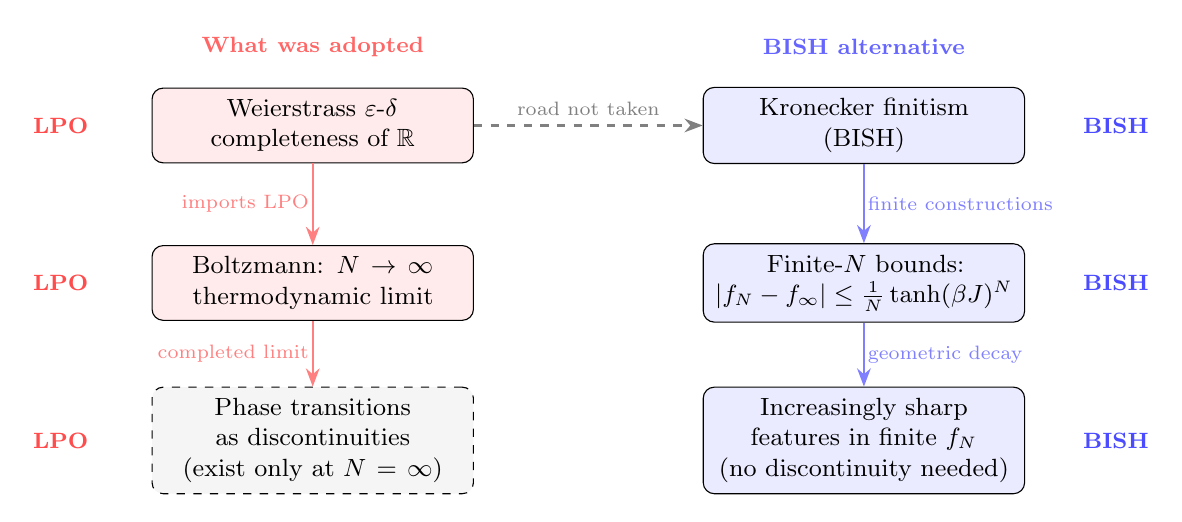
\begin{tikzpicture}[
  >=Stealth,
  every node/.style={font=\small},
  box/.style={draw, rounded corners, minimum height=0.9cm, text width=3.8cm, align=center, inner sep=4pt},
  adopted/.style={box, fill=red!8},
  bish/.style={box, fill=blue!8},
  result/.style={box, fill=gray!8, dashed},
  lbl/.style={font=\scriptsize, midway, fill=white, inner sep=1pt}
]
% Left column: what was adopted
\node[adopted] (weier) at (0, 4) {Weierstrass $\varepsilon$-$\delta$\\completeness of $\mathbb{R}$};
\node[adopted] (boltz) at (0, 2) {Boltzmann: $N \to \infty$\\thermodynamic limit};
\node[result] (phase) at (0, 0) {Phase transitions\\as discontinuities\\(exist only at $N = \infty$)};

% Right column: BISH alternative
\node[bish] (kron) at (7, 4) {Kronecker finitism\\(BISH)};
\node[bish] (finite) at (7, 2) {Finite-$N$ bounds:\\$|f_N - f_\infty| \leq \frac{1}{N}\tanh(\beta J)^N$};
\node[bish] (sharp) at (7, 0) {Increasingly sharp\\features in finite $f_N$\\(no discontinuity needed)};

% Arrows left column
\draw[->, thick, red!50] (weier) -- node[lbl, left] {imports LPO} (boltz);
\draw[->, thick, red!50] (boltz) -- node[lbl, left] {completed limit} (phase);

% Arrows right column
\draw[->, thick, blue!50] (kron) -- node[lbl, right] {finite constructions} (finite);
\draw[->, thick, blue!50] (finite) -- node[lbl, right] {geometric decay} (sharp);

% Cross arrows
\draw[->, thick, dashed, gray] (weier) -- node[above, font=\scriptsize] {road not taken} (kron);

% Labels
\node[font=\footnotesize\bfseries, red!60] at (0, 5) {What was adopted};
\node[font=\footnotesize\bfseries, blue!60] at (7, 5) {BISH alternative};

% Cost labels — offset further from boxes to avoid text mixing
\node[font=\footnotesize\bfseries, red!70, fill=white, inner sep=2pt, rounded corners=1pt] at (-3.2, 4) {LPO};
\node[font=\footnotesize\bfseries, red!70, fill=white, inner sep=2pt, rounded corners=1pt] at (-3.2, 2) {LPO};
\node[font=\footnotesize\bfseries, red!70, fill=white, inner sep=2pt, rounded corners=1pt] at (-3.2, 0) {LPO};
\node[font=\footnotesize\bfseries, blue!70, fill=white, inner sep=2pt, rounded corners=1pt] at (10.2, 4) {BISH};
\node[font=\footnotesize\bfseries, blue!70, fill=white, inner sep=2pt, rounded corners=1pt] at (10.2, 2) {BISH};
\node[font=\footnotesize\bfseries, blue!70, fill=white, inner sep=2pt, rounded corners=1pt] at (10.2, 0) {BISH};

\end{tikzpicture}
\caption{Act~I: the Weierstrass--Boltzmann import.
Weierstrass's completeness of the reals (LPO) was inherited by Boltzmann's thermodynamic limit.
For this exactly solvable model, the BISH alternative---finite-$N$ error bounds with geometric decay---recovers every empirical prediction.
Paper~29 shows this bypass is not available for generic systems: Fekete's lemma ($\equiv$ LPO) is the only route when explicit bounds are unavailable.
The ``road not taken'' from Kronecker finitism was available from the 1870s---but only for tier~1 systems.}
\label{fig:act1-import}
\end{figure}

% ============================================================
\section{Act~II: The Quantum Formalization (1925--1935)}
% ============================================================

Quantum mechanics was born constructive and became classical.

Heisenberg's matrix mechanics (1925) was intrinsically finite-dimensional and algebraic.
Matrices, commutators, trace formulas---the operational toolkit of quantum mechanics is linear algebra, and finite-dimensional linear algebra is BISH to the core.
Schr\"odinger's wave mechanics (1926) introduced infinite-dimensional function spaces, but the actual calculations---the hydrogen atom, the harmonic oscillator---used finite-term power series and explicit formulas.
Dirac's transformation theory (1927) unified matrix and wave mechanics through a powerful notation that also obscured the question of dimension.

A scope note is necessary here.
The constructive calibration programme examines quantum \emph{states}---density matrices, singular states, spectral structure---not quantum \emph{dynamics}.
Time evolution operators, scattering amplitudes, the S-matrix, and path integrals for dynamical processes remain uncalibrated.
The results below concern the static mathematical objects of quantum theory, not the dynamical ones.

Then came von~Neumann.

In 1932, von~Neumann published \emph{Mathematische Grundlagen der Quantenmechanik} \cite{vonNeumann1932}, which axiomatized quantum mechanics in terms of infinite-dimensional Hilbert spaces, the spectral theorem for unbounded self-adjoint operators, and the theory of von~Neumann algebras.
This was a masterwork of mathematical architecture---and a consequential trade.
A finite, operational physical theory was recast in the language of infinite-dimensional functional analysis, gaining enormous conceptual power (general spectral theory, representation theory, the classification of quantum symmetries) at a logical cost that would remain invisible for ninety years.
The physics community gained a thinking tool of extraordinary scope and gradually lost the ability to distinguish the physics from the tool.

Our programme reveals the cost.
The Heisenberg uncertainty principle---arguably the defining statement of quantum mechanics---splits into two logically distinct results \cite{Lee2026g}.
The \emph{preparation uncertainty} inequality (the Robertson-Schr\"odinger bound) states that for any quantum state~$\psi$ with $\|\psi\|=1$ and any pair of observables $A$, $B$:
\begin{equation}\label{eq:rs-inequality}
|\langle \psi, [A,B]\,\psi\rangle|^2 \;\leq\; 4\,\mathrm{Var}_\psi(A)\;\mathrm{Var}_\psi(B),
\end{equation}
where $\mathrm{Var}_\psi(A) = \|A\psi - \langle A\rangle\psi\|^2$ and $[A,B] = AB - BA$.
This is fully constructive: the proof centers the state, applies the Cauchy-Schwarz inequality to the inner product $\langle \Delta_A\psi, \Delta_B\psi\rangle$, and decomposes the result into commutator and anticommutator contributions.
Pure Hilbert space geometry---BISH.
The \emph{measurement uncertainty} form---which concerns the statistics extracted from repeated measurements---requires Dependent Choice, a modest extension that allows countable sequences of dependent selections.
The physical core of quantum uncertainty needs no classical logic.
The classical overhead enters only when you extract statistical information from infinite measurement sequences.

This separation has a deeper significance than a technical footnote about choice principles.
The Born rule---the postulate that measurement probabilities equal $|\langle\lambda|\psi\rangle|^2$---is itself an idealization.
It asserts that relative frequencies over infinitely many measurements converge to definite probabilities; that convergence is where Dependent Choice enters.
The geometric content of quantum mechanics---that a single state cannot be simultaneously sharp in non-commuting observables---is BISH, a property of one vector in a finite-dimensional Hilbert space requiring no measurements at all.
The statistical content---that repeated measurements yield frequencies approaching the Born probabilities---requires the construction of infinite measurement sequences and the extraction of their limits.
Quantum mechanics thus splits into two logical layers: a constructive geometric core (preparation uncertainty, Cauchy--Schwarz, BISH) and a statistical superstructure (measurement uncertainty, the Born rule, Dependent Choice).
The physical core that makes quantum mechanics \emph{strange}---superposition, interference, non-commutativity---needs no idealization.
The apparatus that makes quantum mechanics \emph{predictive} over infinite ensembles does.

The distinction between physical states and mathematical artifacts is even sharper.
In quantum mechanics, physical states are represented by density matrices---positive operators of unit trace on the Hilbert space.
But the mathematical dual of the trace-class operators contains objects that are \emph{not} density matrices: the \emph{singular states}, functionals that vanish on all compact operators and detect only behavior at spatial infinity.
No laboratory has ever prepared a singular state, because doing so would require controlling infinitely many degrees of freedom simultaneously.

Our programme shows that the mere non-reflexivity of the state space---the fact that singular states ``cannot be ruled out''---is provable in BISH \cite{Lee2026b}.
But \emph{constructively exhibiting} a singular state, with explicit separation data from the space of density matrices, requires WLPO \cite{Lee2026a}.
The gap between ``cannot rule out'' and ``can exhibit'' is precisely the WLPO boundary.
Singular states are cities that appear on the map but have no corresponding settlement in the territory.

Most strikingly, the research programme establishes that Bell nonlocality---the phenomenon that makes quantum mechanics genuinely non-classical---requires no classical logic at all \cite{Lee2026paper11}.
The Tsirelson bound on the CHSH correlations decomposes algebraically: define the CHSH operator
\begin{equation}\label{eq:chsh}
\mathcal{C} \;=\; A \otimes (B + B') \;+\; A' \otimes (B - B')
\end{equation}
where $A, A', B, B'$ are self-adjoint involutions ($A^2 = I$, etc.)\ on $\mathbb{C}^2$.
Because involutions preserve norms, $\|\mathcal{C}\psi\|^2 \leq \|(B+B')\psi_B\|^2 + \|(B-B')\psi_B\|^2$, and the identity $(B+B')^2 + (B-B')^2 = 4I$ yields:
\[
|\langle \psi, \mathcal{C}\psi\rangle| \;\leq\; 2\sqrt{2}.
\]
This is the Tsirelson bound---a theorem of finite-dimensional linear algebra: $4\times 4$ matrices, a sum-of-squares identity, and the parallelogram inequality.
The proof is BISH.
The most distinctively quantum phenomenon needs the least logical strength.

A subtlety emerges when we pass from the \emph{bound} to the \emph{disjunction}.
Bell's theorem refutes local hidden variables constructively---the violation of the CHSH inequality is a BISH fact.
But the physicist's conclusion---``either locality fails \emph{or} realism fails''---is a disjunction on infinite-dimensional objects, and asserting it costs LLPO \cite{Lee2026paper21}.
The same LLPO cost governs Kochen-Specker contextuality \cite{Lee2026paper24}.
Bell nonlocality involves spatially separated systems; KS contextuality involves a single system.
They are physically distinct phenomena.
Yet both cost LLPO for the same structural reason: disjunction without constructive witness.
The constructive hierarchy identifies them as the same logical phenomenon in different physical clothing---a structural identity invisible to informal physical analysis, detected only because the proof assistant forces logical bookkeeping at a scale and precision that informal methods were not designed to track.
This is a first hint that the hierarchy between WLPO and LPO is physically populated, a point we return to in Section~\ref{sec:thesis}.

The spectrum itself---the central mathematical object of quantum mechanics, the set of possible measurement outcomes for an observable---is an idealization.
An experimentalist measures finitely many energy levels to finite precision: the hydrogen Lyman series, a handful of absorption lines, each located within instrumental error bars.
That is BISH\@.
The assertion that a specific value $\lambda$ belongs \emph{exactly} to the spectrum of an operator~$H$---rather than merely within~$\varepsilon$ of the spectrum for every~$\varepsilon > 0$---requires Markov's Principle \cite{Lee2026f}.
The full spectral theorem, guaranteeing a complete projection-valued measure decomposing any self-adjoint operator into spectral subspaces, requires substantially more.
The most fundamental mathematical structure of quantum mechanics---the object from which every measurement prediction flows---has a precisely calibrated logical cost, and the physical content accessible to a finite observer sits below that cost at BISH\@.

Taken together, the quantum calibrations reveal a layered architecture.
Von~Neumann's 1932 formalization introduced not one but several measurable layers of idealization above BISH: the Born rule's convergence of measurement statistics (Dependent Choice, \cite{Lee2026g}), exact spectral membership (Markov's Principle, \cite{Lee2026f}), the disjunctive content of Bell's theorem and Kochen-Specker contextuality (LLPO, \cite{Lee2026paper21, Lee2026paper24}), the existence of singular states in the bidual (WLPO, \cite{Lee2026a}), and the variational minimum of a continuous function on a compact domain (Fan Theorem, \cite{Lee2026paper23}).
Each layer has a machine-verified logical cost.
Each separates physical content from mathematical infrastructure.
The pattern is uniform: what a finite observer can prepare, measure, and record is BISH; each assertion about completed infinities---infinite measurement sequences, exact set membership, functionals on infinite-dimensional duals---costs a specific, independently identifiable non-constructive principle.

\textbf{The constructive alternative.}
It was not merely available---it was actively contested.
Brouwer's intuitionism was at its most creative precisely during the decade (1920--1930) when quantum mechanics was being formalized.
In 1928, the year Dirac published his equation and von~Neumann began his axiomatization, Hilbert had Brouwer expelled from the editorial board of \emph{Mathematische Annalen}---marginalizing intuitionism at the very moment the quantum formalism was hardening \cite{vanDalen2005}.
A decade earlier, Hermann Weyl had published \emph{Das Kontinuum} (1918) \cite{Weyl1918}, constructing a predicative foundation for analysis explicitly intended for physical application.
Weyl abandoned this programme under social pressure from the Hilbert school, not because of any mathematical inadequacy.
Most remarkably, von~Neumann himself grew dissatisfied with the Hilbert space formalism within a few years and turned to finite type~II$_1$ factors---where the pathologies of unbounded operators and non-reflexivity vanish \cite{Redei1996}.
The architect of the cathedral privately preferred the cellar.

\begin{figure}[ht]
\centering
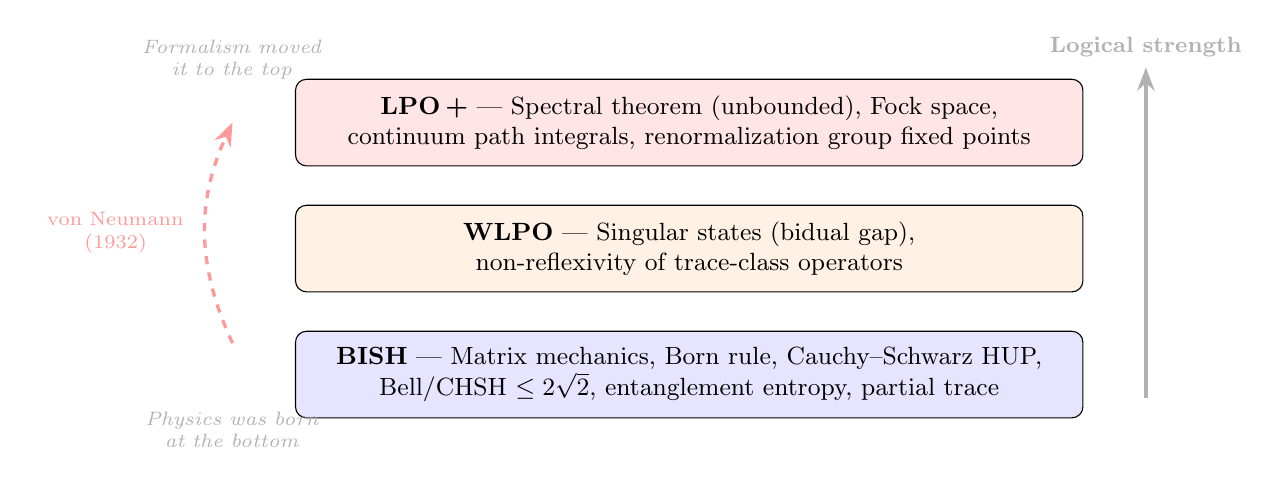
\begin{tikzpicture}[
  >=Stealth,
  every node/.style={font=\small},
  layer/.style={draw, minimum width=10cm, minimum height=1.1cm, align=center, inner sep=3pt}
]
% Bottom layer: BISH
\node[layer, fill=blue!10, rounded corners] (bish) at (0, 0)
  {\textbf{BISH} --- Matrix mechanics, Born rule, Cauchy--Schwarz HUP,\\
   Bell/CHSH $\leq 2\sqrt{2}$, entanglement entropy, partial trace};
% Middle layer: WLPO
\node[layer, fill=orange!10, rounded corners] (wlpo) at (0, 1.6)
  {\textbf{WLPO} --- Singular states (bidual gap),\\
   non-reflexivity of trace-class operators};
% Top layer: LPO+
\node[layer, fill=red!10, rounded corners] (lpo) at (0, 3.2)
  {\textbf{LPO\,+} --- Spectral theorem (unbounded), Fock space,\\
   continuum path integrals, renormalization group fixed points};

% Arrow on right
\draw[->, very thick, gray!60] (5.8, -0.3) -- (5.8, 3.9)
  node[above, font=\footnotesize\bfseries, gray!60] {Logical strength};

% Von Neumann arrow
\draw[->, very thick, red!40, dashed] (-5.8, 0.4) to[bend left=25]
  node[left, font=\scriptsize, text width=2cm, align=center] {von Neumann\\(1932)} (-5.8, 3.2);

% Annotation
\node[font=\scriptsize\itshape, gray!60, text width=4cm, align=center] at (-5.8, -0.7)
  {Physics was born\\at the bottom};
\node[font=\scriptsize\itshape, gray!60, text width=4cm, align=center] at (-5.8, 4.0)
  {Formalism moved\\it to the top};

\end{tikzpicture}
\caption{Act~II: the quantum formalization.
Heisenberg's matrix mechanics (1925) is BISH\@.
Von~Neumann's Hilbert space axiomatization (1932) moved the formalism to infinite dimensions.
The empirical content---uncertainty relations, Bell nonlocality, entanglement entropy---remains at BISH\@.
Singular states (WLPO) are mathematical artifacts of the infinite-dimensional framework.
For the LPO+ layer, Paper~29 shows the picture is more nuanced: the thermodynamic limit and singularity theorems are ineliminable (tier~3), not merely organizational.}
\label{fig:quantum-layers}
\end{figure}

\begin{keymessage}
Quantum mechanics was born constructive (matrix mechanics = BISH).
Von~Neumann moved it to infinite dimensions (1932).
The HUP, Bell/CHSH, and entanglement entropy are all BISH; singular states cost WLPO\@.
The empirical content stayed at sea level; only the formalism ascended.
\end{keymessage}

% ============================================================
\section{Act~III: The Singularity Detour (1939--1970)}
% ============================================================

In 1939, Einstein published a paper arguing that gravitational collapse could not produce singularities---points of infinite curvature where the equations of general relativity break down \cite{Einstein1939}.
His conviction was principled: ``Every field theory, in our opinion, must therefore adhere to the fundamental principle that singularities of the field are to be excluded.''
Infinite curvature at a point, he reasoned, is not something the physical world produces.
It is a mathematical pathology, an artifact of pushing the formalism past its domain of validity.

The same year, Oppenheimer and Snyder published a paper showing that for a sufficiently massive star, gravitational collapse is inevitable \cite{OppenheimerSnyder1939}.
The community sided with Oppenheimer.
Then, in 1965, Penrose proved the first singularity theorem \cite{Penrose1965}: under generic conditions---trapped surfaces, reasonable energy conditions, global hyperbolicity---spacetime is geodesically incomplete.
Incomplete geodesics are the mathematical signature of singularities.
Hawking extended the result, and the Hawking-Penrose theorems (1970) established singularities as an inescapable feature of general relativity.
Einstein, who died in 1955, was posthumously declared wrong.

Our framework reaches a conclusion that partially aligns with his, though for entirely different reasons he could not have articulated, and with an important qualification he could not have anticipated.
His 1939 argument was physically flawed---it relied on circular orbit stability, which is irrelevant to radial collapse---but his instinct that the singularity marks a boundary of the formalism rather than a feature of the world finds partial support in the constructive analysis, which locates the completed-limit assertion precisely at the LPO boundary.
The qualification is this: Paper~29 shows that LPO-level reasoning is sometimes ineliminable.
The singularity theorem, like the thermodynamic limit, is an instance of \emph{productive} LPO---it enables the entire programme of black hole physics.
Whether the singularity is ``merely'' a formal artifact or describes something physically real is a question the programme reframes but does not settle: the \emph{mathematical} description of geodesic incompleteness requires LPO, and Paper~29 shows that requirement cannot be eliminated.

The Penrose singularity theorem has the following logical structure.
The Raychaudhuri equation \cite{Raychaudhuri1955} governs the evolution of the expansion scalar $\theta$ along a geodesic congruence:
\begin{equation}\label{eq:raychaudhuri}
\frac{d\theta}{d\tau} \;=\; -\frac{1}{3}\theta^2 \;-\; \sigma_{\mu\nu}\sigma^{\mu\nu} \;+\; \omega_{\mu\nu}\omega^{\mu\nu} \;-\; R_{\mu\nu}\,u^\mu u^\nu,
\end{equation}
where $\sigma_{\mu\nu}$ is the shear tensor, $\omega_{\mu\nu}$ is the vorticity, $R_{\mu\nu}$ is the Ricci tensor, and $u^\mu$ is the tangent vector.
When the strong energy condition holds ($R_{\mu\nu}u^\mu u^\nu \geq 0$) and vorticity vanishes, the right-hand side is non-positive: the expansion decreases monotonically.
This is a first-order ordinary differential equation on finite parameter intervals---\emph{BISH}.
(The equation displayed is the \emph{timelike} Raychaudhuri equation; Penrose's 1965 theorem uses the \emph{null} version, with $\tfrac{1}{2}\theta^2$ replacing $\tfrac{1}{3}\theta^2$ and vanishing vorticity guaranteed by the twist-free hypothesis on the null geodesic congruence.
The logical structure---finite ODE at BISH, completed limit at LPO---is identical in both cases.)

The non-constructive step comes at the end, and it is the same step as in the thermodynamic limit.
The Penrose theorem asserts a dichotomy on the monotonically decreasing expansion scalar: either the geodesic terminates at finite parameter value (singularity) or it extends forever.
This is Bounded Monotone Convergence---LPO \cite{BridgesVita2006}.
The physical content of the singularity theorem is the Raychaudhuri focusing, which is BISH.
The Kretschmann curvature invariant $K = 48M^2/r^6$ is constructively computable for any $r > 0$, and its divergence is constructively witnessable: for any bound~$B$, one can constructively exhibit~$r_0 > 0$ with $K(r_0) > B$.
This unbounded growth is BISH---not a completed limit.
The completed-limit content resides in the assertion that the geodesic actually \emph{reaches} $r = 0$: that a bounded monotone decreasing sequence of radial coordinates converges to a definite real number.
This is the same bounded monotone convergence equivalence (BMC~$\equiv$~LPO) as in the thermodynamic limit \cite{Lee2026paper13}.
The physics is the focusing; the singularity is where the map's logical resources escalate from BISH to LPO\@.
Whether the territory ``just keeps going'' or the LPO-level description captures something physically real is precisely the question that the three-tier hierarchy reframes: at tier~3, the map's non-constructive resources are not idle but ineliminable.

Paper~13 \cite{Lee2026paper13} formalizes this decomposition for the Schwarzschild case.
The event horizon at $r = 2M$ serves as a \emph{logical boundary}: the exterior geometry (Paper~1) and the interior's finite-time physics---the cycloid geodesic reaching $r = 0$ at proper time $\tau^* = \pi M$, the Kretschmann scalar's constructively witnessable divergence---are BISH.
Only the completed-limit assertion that every bounded monotone trajectory converges to a definite real costs LPO.
The horizon demarcates what can be asserted without surveying an infinite set.

The BMC~$\equiv$~LPO equivalence extends beyond geodesic incompleteness to a fifth physical domain.
Paper~17 \cite{Lee2026paper17} establishes that the Bekenstein-Hawking entropy---$S_{\mathrm{BH}} = A/(4\ell_P^2)$, the entropy assigned to a black hole proportional to its horizon area---is constructively computable for any finite discretization.
But asserting that the entropy per unit area \emph{converges} to the Bekenstein-Hawking value as the discretization is refined costs LPO, through the same bounded monotone convergence mechanism.
Statistical mechanics (Paper~8), general relativity (Paper~13), wave function collapse (Paper~14), Noether's theorem for infinite systems (Paper~15), and now black hole thermodynamics (Paper~17) all pay the same logical price for the same abstract operation: passing from a bounded monotone sequence to its completed limit.
Five domains, one principle.
Paper~29 \cite{Lee2026paper29Fekete} identifies the generic mechanism behind this five-domain pattern.
Each domain produces a subadditive quantity; Fekete's Subadditive Lemma is the tool that extracts its limit; and Fekete $\equiv$ LPO\@.
The five-domain coincidence is not coincidence---it is the logical cost of subadditivity itself.

\textbf{The constructive perspective.}
Einstein was not alone in his discomfort.
Eddington found singularities ``repugnant'' and publicly attacked Chandrasekhar's mass limit calculations in 1935.
The Raychaudhuri equation itself---the constructive core of the singularity theorems---provides all the physical content: quantitative bounds on geodesic convergence over finite parameter intervals.
Every numerical relativity simulation operates at this BISH level, computing finite-precision approximations to geodesic behavior without asserting completed limits---from binary black hole merger simulations to gravitational wave template generation, all finite-precision computations on finite grids.
As recently as 2023, Roy Kerr---discoverer of the Kerr metric for rotating black holes---has argued that physical black holes need not contain singularities \cite{Kerr2023}.
The constructive analysis partially aligns with this persistent minority view: the finite-time physics is BISH, and the completed-limit assertion is the escalation point.
But the programme's own results counsel against declaring the singularity a mere artifact.
The singularity theorem, like the thermodynamic limit, is an instance of productive LPO---it generates predictions (the existence of trapped regions, the inevitability of collapse under generic energy conditions) that have been confirmed by gravitational wave observations of merging black holes.
The correct conclusion is not that singularities are ``unreal'' but that the question of their reality is entangled with the question of which logical principles describe nature at infinite limits---a question the programme reframes but does not resolve.

\begin{figure}[ht]
\centering
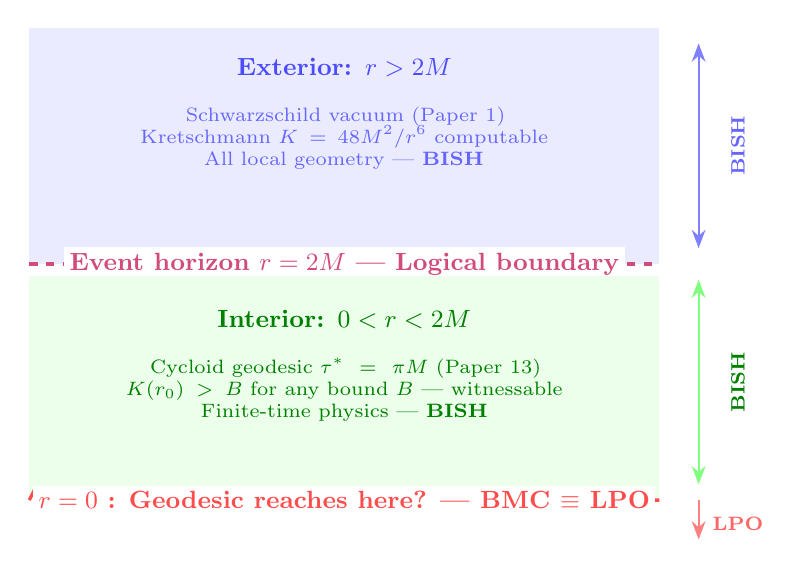
\begin{tikzpicture}[
  >=Stealth,
  every node/.style={font=\small}
]
% Exterior region
\fill[blue!8] (-4, 0) rectangle (4, 3);
\node[font=\small\bfseries, blue!70] at (0, 2.5) {Exterior: $r > 2M$};
\node[font=\scriptsize, blue!60, text width=6cm, align=center] at (0, 1.6)
  {Schwarzschild vacuum (Paper~1)\\Kretschmann $K = 48M^2/r^6$ computable\\All local geometry --- \textbf{BISH}};

% Event horizon
\draw[very thick, dashed, purple!70] (-4, 0) -- (4, 0);
\node[font=\small\bfseries, purple!70, fill=white, inner sep=2pt] at (0, 0) {Event horizon $r = 2M$ --- Logical boundary};

% Interior region
\fill[green!8] (-4, -3) rectangle (4, -0.15);
\node[font=\small\bfseries, green!50!black] at (0, -0.7) {Interior: $0 < r < 2M$};
\node[font=\scriptsize, green!50!black, text width=6.5cm, align=center] at (0, -1.6)
  {Cycloid geodesic $\tau^* = \pi M$ (Paper~13)\\$K(r_0) > B$ for any bound $B$ --- witnessable\\Finite-time physics --- \textbf{BISH}};

% Singularity
\draw[very thick, red!70, decorate, decoration={zigzag, segment length=6pt, amplitude=3pt}]
  (-4, -3) -- (4, -3);
\node[font=\small\bfseries, red!70, fill=white, inner sep=2pt] at (0, -3)
  {$r = 0$ : Geodesic reaches here? --- \textbf{BMC $\equiv$ LPO}};

% Right-side labels
\draw[thick, blue!50, <->] (4.5, 0.2) -- (4.5, 2.8);
\node[font=\scriptsize\bfseries, blue!60, rotate=90] at (5.0, 1.5) {BISH};
\draw[thick, green!50, <->] (4.5, -2.8) -- (4.5, -0.2);
\node[font=\scriptsize\bfseries, green!50!black, rotate=90] at (5.0, -1.5) {BISH};
\draw[thick, red!50, ->] (4.5, -3.0) -- (4.5, -3.5);
\node[font=\scriptsize\bfseries, red!60] at (5.0, -3.3) {LPO};

\end{tikzpicture}
\caption{Act~III: the event horizon as a logical boundary.
The exterior geometry and the interior's finite-time physics are both BISH\@.
The singularity---the assertion that a bounded monotone trajectory converges to a definite real---costs LPO\@.
The horizon demarcates what can be asserted without surveying an infinite set (Paper~13).}
\label{fig:blackhole}
\end{figure}

\begin{keymessage}
The Raychaudhuri focusing equation is BISH\@.
The Kretschmann divergence is constructively witnessable.
The assertion ``the geodesic reaches $r = 0$'' costs LPO---the same BMC equivalence as the thermodynamic limit.
Paper~29 shows this LPO cost is ineliminable: geodesic incompleteness, like the thermodynamic limit, is productive non-constructive mathematics.
The event horizon is a logical boundary (Paper~13).
\end{keymessage}

% ============================================================
\section{Act~IV: The Greatest Predictions from the Smallest Logic (1947--1975)}
% ============================================================

Between 1947 and 1975, quantum field theory delivered the cellar-and-cathedral pattern of Section~1 at industrial scale.
Every Feynman diagram computation---the actual source of QFT's legendary precision---is BISH: finite integrals, finite arithmetic, controlled error.
But the formalism grew a new cathedral above the cellar.
Fock space completeness, renormalization group fixed points, and the vacuum state all live at LPO or beyond.
And the path integral---a formal ``integral'' over an infinite-dimensional configuration space for which no rigorous measure exists---requires choice principles far stronger still.

Yet the predictions are spectacular.
The formalism works---not because the infinite-dimensional apparatus is physically real, but because it is an effective mnemonic for organizing BISH-level computations.
The path integral is a beautiful legend on the map explaining how to read the contour lines.
The contour lines---the Feynman diagrams---are the actual geography.
There is an irony here that deserves acknowledgment.
The Wilsonian renormalization group---itself an LPO-level construction, since its fixed points live in an infinite-dimensional space of theories---is precisely the framework that explains \emph{why} the cellar is stable: it shows that high-energy physics decouples from low-energy predictions, justifying the truncation to finite loop order.
The cathedral's most important structural insight is the proof that the cellar is self-sufficient.

The Yang-Mills mass gap problem---one of the seven Clay Millennium Prize Problems---asks for a proof that a quantum field theory satisfying certain axioms has a positive mass gap.
The axioms involve infinite-dimensional structures (Wightman axioms, Osterwalder-Schrader axioms) that are LPO or stronger.
If the empirical content of Yang-Mills theory is BISH---and lattice QCD already computes hadron masses from first principles at BISH---the Millennium Problem asks for a rigorous construction of Yang-Mills in the \emph{continuum limit}, connecting the BISH-level lattice computation to the LPO-level continuum formalism.
The Millennium Problem asks whether the map (continuum formalization) matches the territory (lattice computations) in a specific rigorous sense.
The lattice predictions---hadron masses, the proton charge radius---do not wait for the answer; they are already confirmed at BISH\@.
But the existence or non-existence of the continuum limit is a question about the mathematical infrastructure, not about the physical phenomena that infrastructure was built to describe.

Not every non-constructive scaffold is idle, however---some are idle and \emph{known} to be idle.
Paper~18 \cite{Lee2026paper18} tests the \emph{Scaffolding Principle} on the Standard Model's Yukawa RG. Numerical investigations (Phases~A--B) show 1/10 positive: the infrared dynamics do not determine the mass hierarchy. A Lean~4 formalization (Phase~C, 902 lines) reveals a sharp constructive stratification: the one-loop RG flow is BISH, step-function threshold decoupling costs WLPO, and CKM eigenvalue-crossing detection costs LPO. The mass hierarchy is a genuine structural feature, not an artifact of classical logic---but the textbook formalism carries non-trivial constructive cost.

\textbf{The constructive alternative.}
The fragility of the formalism was recognized from within. Dyson showed in 1952 \cite{Dyson1952} that the QED perturbation series diverges---it is asymptotic, not convergent. Haag's theorem (1955) \cite{Haag1996} demonstrated that the infinity of inequivalent Fock space representations is an artifact of infinite dimensions. The Glimm-Jaffe programme \cite{GlimmJaffe1981} built rigorous QFT in two and three spacetime dimensions; the four-dimensional case remains open (the Millennium Prize). Every actual prediction---lattice QCD hadron masses, QED magnetic moments---is a finite computation at BISH\@. The constructive alternative is what physicists already do.

\begin{figure}[ht]
\centering
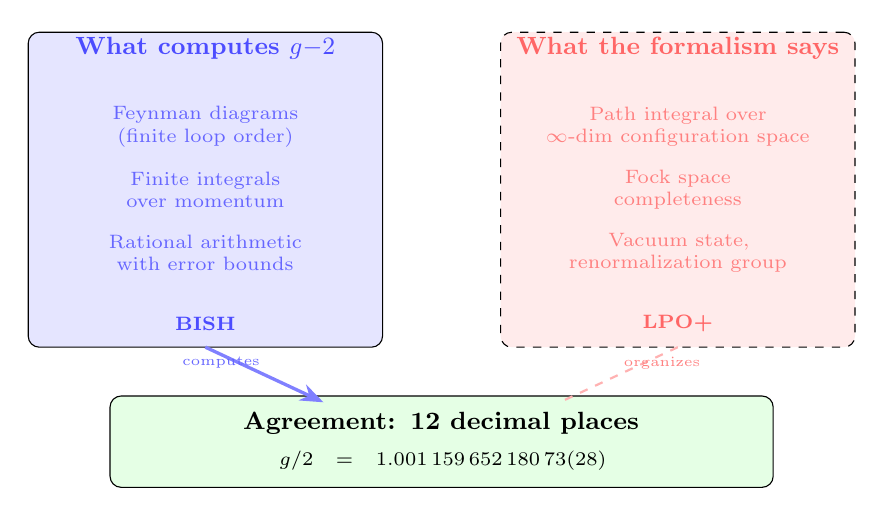
\begin{tikzpicture}[
  >=Stealth,
  every node/.style={font=\small},
  col/.style={draw, rounded corners, minimum width=4.5cm, align=center, inner sep=6pt}
]
% Left column: what actually computes
\node[col, fill=blue!10, minimum height=4cm] (cellar) at (-3, 2) {};
\node[font=\small\bfseries, blue!70] at (-3, 3.8) {What computes $g{-}2$};
\node[font=\scriptsize, blue!60, text width=3.8cm, align=center] at (-3, 2.8)
  {Feynman diagrams\\(finite loop order)};
\node[font=\scriptsize, blue!60, text width=3.8cm, align=center] at (-3, 2.0)
  {Finite integrals\\over momentum};
\node[font=\scriptsize, blue!60, text width=3.8cm, align=center] at (-3, 1.2)
  {Rational arithmetic\\with error bounds};
\node[font=\scriptsize\bfseries, blue!70] at (-3, 0.3) {BISH};

% Right column: the formalism
\node[col, fill=red!8, minimum height=4cm, dashed] (cath) at (3, 2) {};
\node[font=\small\bfseries, red!60] at (3, 3.8) {What the formalism says};
\node[font=\scriptsize, red!50, text width=3.8cm, align=center] at (3, 2.8)
  {Path integral over\\$\infty$-dim configuration space};
\node[font=\scriptsize, red!50, text width=3.8cm, align=center] at (3, 2.0)
  {Fock space\\completeness};
\node[font=\scriptsize, red!50, text width=3.8cm, align=center] at (3, 1.2)
  {Vacuum state,\\renormalization group};
\node[font=\scriptsize\bfseries, red!60] at (3, 0.3) {LPO+};

% Result
\node[draw, rounded corners, fill=green!10, font=\small\bfseries, text width=8cm, align=center, inner sep=6pt]
  (result) at (0, -1.2) {Agreement: 12 decimal places\\[2pt]
  \normalfont\scriptsize $g/2 = 1.001\,159\,652\,180\,73(28)$};

% Arrow from cellar to result
\draw[->, very thick, blue!50] (-3, 0) -- (-1.5, -0.7);
% Disconnected from cathedral
\draw[thick, red!30, dashed] (3, 0) -- (1.5, -0.7);
\node[font=\tiny, red!50] at (2.8, -0.2) {organizes};
\node[font=\tiny, blue!60] at (-2.8, -0.2) {computes};

\end{tikzpicture}
\caption{Act~IV: the most precise prediction in physics.
The $g{-}2$ computation uses finite Feynman diagrams (BISH, solid arrow).
The infinite-dimensional formalism (LPO+, dashed) organizes the computation
but does not contribute to the numerical result.
Twelve decimal places of agreement come from the cellar, not the cathedral.
For tier~3 systems (generic phase transitions), Paper~29 shows the cathedral is not merely organizational---Fekete's lemma ($\equiv$ LPO) is the only route to the thermodynamic limit.}
\label{fig:g-minus-2}
\end{figure}

% ============================================================
\section{Act~V: The Interpretive Crisis (1975--Present)}
% ============================================================

After the Standard Model was completed in the mid-1970s, the data stream slowed.
The model agreed with every experiment.
New phenomena required higher energies, bigger accelerators, longer timescales, and more money.
Theorists, no longer constrained by a steady flow of surprises from the laboratory, began exploring the mathematical formalism itself.

What they explored was the non-constructive superstructure.

String theory posits a landscape of $10^{500}$ vacuum states---solutions to the equations of the theory that represent possible universes \cite{BoussoPolchinski2000, Susskind2003}.
This is an assertion about the structure of an infinite-dimensional space of solutions.
No finite experiment can probe it.
The many-worlds interpretation of quantum mechanics takes the universal wave function literally, asserting the real physical existence of a branching structure in infinite-dimensional Hilbert space.
No measurement can access the other branches.
The black hole information paradox asks what happens to quantum information at a singularity---combining two LPO-level idealizations (the singularity and the infinite-dimensional state space) into a single problem \cite{AMPS2013}.

From the constructive hierarchy's perspective, these debates share a structural feature: they appear to concern mathematical objects at LPO or higher, without having produced BISH-level predictions that connect back to experiment.

A caveat is essential: the programme has not formally calibrated the string landscape, the multiverse, or the information paradox.
Those programmes have not been formalized in Lean~4, and no constructive reverse mathematics result establishes their logical level.
The observation that they have produced no BISH-level predictions is an empirical fact about the current state of theoretical physics, not a theorem about logical structure.
It is possible---though no one has demonstrated it---that future developments in string theory could yield specific finite-precision predictions at BISH\@.
What the programme \emph{can} say formally is this: the logical level alone does not determine whether a programme is productive.
Paper~29 shows that LPO does real physical work at phase transitions (tier~3), and the singularity theorems require LPO for geodesic incompleteness (Paper~13).
The thermodynamic limit costs LPO but produces specific free energies and critical exponents.
These are examples of \emph{productive} non-constructive mathematics---LPO-level reasoning that generates BISH-level predictions confirmed by experiment.
The string landscape has not, to date, produced analogous predictions; but whether this is an intrinsic feature of its logical structure or a contingent failure of the current programme is an open question that CRM could in principle address but has not yet.

This diagnosis differs from existing critiques---Hossenfelder blaming aesthetics, Woit unfalsifiability, Smolin sociology.
Ours identifies a \emph{structural} observation: the calibrated programmes that produce confirmed predictions operate at BISH; the uncalibrated programmes that have not produced confirmed predictions appear to operate at higher logical levels.
The correlation is suggestive but not yet a theorem.
The formalism is not necessarily wrong; it may be \emph{idle}---machinery not connected to any output---or it may be productive in ways not yet demonstrated.
The distinction between ``productive LPO'' (thermodynamic limit, singularity theorems) and what appears to be ``idle LPO+'' (landscape, multiverse) is the programme's conjecture, not its calibration result.

A qualification is essential.
Not all post-1975 theoretical work explores the non-constructive superstructure.
Lattice QCD (building on Wilson's 1974 construction \cite{Wilson1974}) has matured into a BISH-level computational programme that predicts hadron masses to percent-level accuracy.
Effective field theory (Weinberg, 1979 onward) organizes finite-order calculations systematically without claiming convergence of the full perturbation series.
Tensor network methods (White 1992, Vidal 2003 onward) provide finite-dimensional variational approaches to quantum many-body systems that avoid infinite-dimensional Hilbert spaces entirely.
Validated numerics and computer-assisted proofs employ interval arithmetic at BISH.
The diagnosis targets specifically those programmes---the string landscape, the multiverse, the information paradox---that operate at logical levels inherently disconnected from finite experiment.
The idle machinery is not ``all post-1975 theory'' but the subset that explores the non-constructive superstructure without producing BISH-level predictions.

\begin{figure}[ht]
\centering
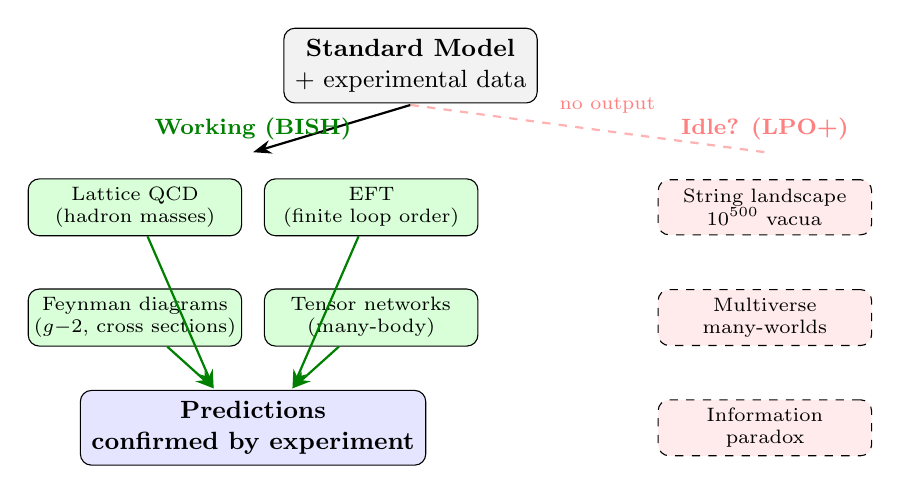
\begin{tikzpicture}[
  >=Stealth,
  every node/.style={font=\small},
  gear/.style={draw, rounded corners, minimum height=0.7cm, align=center, inner sep=3pt, font=\scriptsize}
]
% Input
\node[draw, rounded corners, fill=gray!10, minimum width=3cm, align=center, inner sep=4pt]
  (input) at (0, 3.0) {\textbf{Standard Model}\\+ experimental data};

% Working machinery (BISH)
\node[gear, fill=green!15, text width=2.5cm] (lqcd) at (-3.5, 1.2) {Lattice QCD\\(hadron masses)};
\node[gear, fill=green!15, text width=2.5cm] (eft) at (-0.5, 1.2) {EFT\\(finite loop order)};
\node[gear, fill=green!15, text width=2.5cm] (feyn) at (-3.5, -0.2) {Feynman diagrams\\($g{-}2$, cross sections)};
\node[gear, fill=green!15, text width=2.5cm] (tensor) at (-0.5, -0.2) {Tensor networks\\(many-body)};

% Idle machinery (LPO+)
\node[gear, fill=red!8, dashed, text width=2.5cm] (string) at (4.5, 1.2) {String landscape\\$10^{500}$ vacua};
\node[gear, fill=red!8, dashed, text width=2.5cm] (multi) at (4.5, -0.2) {Multiverse\\many-worlds};
\node[gear, fill=red!8, dashed, text width=2.5cm] (info) at (4.5, -1.6) {Information\\paradox};

% Output
\node[draw, rounded corners, fill=blue!10, minimum width=3cm, align=center, inner sep=4pt, font=\small\bfseries]
  (output) at (-2, -1.6) {Predictions\\confirmed by experiment};

% Arrows
\draw[->, thick] (0, 2.5) -- (-2, 1.9);
\draw[->, thick, green!50!black] (lqcd) -- (-2.5, -1.1);
\draw[->, thick, green!50!black] (eft) -- (-1.5, -1.1);
\draw[->, thick, green!50!black] (feyn) -- (-2.5, -1.1);
\draw[->, thick, green!50!black] (tensor) -- (-1.5, -1.1);

% No connection from idle
\draw[thick, red!30, dashed] (0, 2.5) -- (4.5, 1.9);
\node[font=\scriptsize, red!50] at (2.5, 2.5) {no output};

% Labels
\node[font=\footnotesize\bfseries, green!50!black] at (-2, 2.2) {Working (BISH)};
\node[font=\footnotesize\bfseries, red!50] at (4.5, 2.2) {Idle? (LPO+)};

\end{tikzpicture}
\caption{Act~V: working machinery vs.\ idle machinery.
Post-1975 physics divides into programmes that produce BISH-level predictions confirmed by experiment
(left, green) and programmes that explore the non-constructive superstructure without
empirical output (right, red/dashed).
The observation is structural: the programmes that have not produced confirmed predictions appear to operate at higher logical levels than those that have.
Paper~29 qualifies this picture: for generic systems near phase transitions (tier~3), the thermodynamic limit costs LPO ineliminably---not all non-constructive machinery is idle. The idle--working distinction tracks programme-level empirical output, not logical level per se. The string landscape has not been formally calibrated by CRM.}
\label{fig:idle-machinery}
\end{figure}

The constructive hierarchy suggests a diagnosis and a remedy: the next breakthrough may require \emph{less} logical structure, not more---the identification of which parts of the existing formalism are physically idle and their careful removal.

\textbf{The constructive alternative.}
Bishop (1967) \cite{Bishop1967} proved that analysis survives constructively; Gisin (2019--) \cite{Gisin2020, Gisin2021} argues that real numbers are ``the hidden variables of classical physics'' and that intuitionistic mathematics is the natural language for finite systems.
Our programme supplies the formal precision these visions lacked (see Section~\ref{sec:thesis}).

\begin{keymessage}
Programmes that have produced confirmed predictions operate at BISH (lattice QCD, EFT, tensor networks) or at LPO with BISH-level output (thermodynamic limit, singularity theorems).
Programmes that have not produced confirmed predictions---the string landscape, the multiverse, the information paradox---appear to operate at LPO+ without BISH-level output.
The correlation is suggestive but not yet a calibration result: CRM has not formally assessed these programmes.
Paper~29 shows that operating at LPO is not inherently unproductive---the thermodynamic limit costs LPO ineliminably (tier~3) and does real physical work.
\end{keymessage}


% ============================================================
\section{The Logical Geography: What the Proofs Show}
% ============================================================

The preceding narrative rests on a specific body of evidence: a calibration table mapping layers of mathematical physics to their precise position in the constructive hierarchy.
Each entry is machine-verified in the Lean~4 proof assistant, using either constructive reverse mathematics (CRM) over the Mathlib library \cite{Ishihara2006, BridgesVita2006} or an axiom-calibration framework in standalone Lean.

\begin{figure}[ht]
\centering
\resizebox{0.92\textwidth}{!}{%
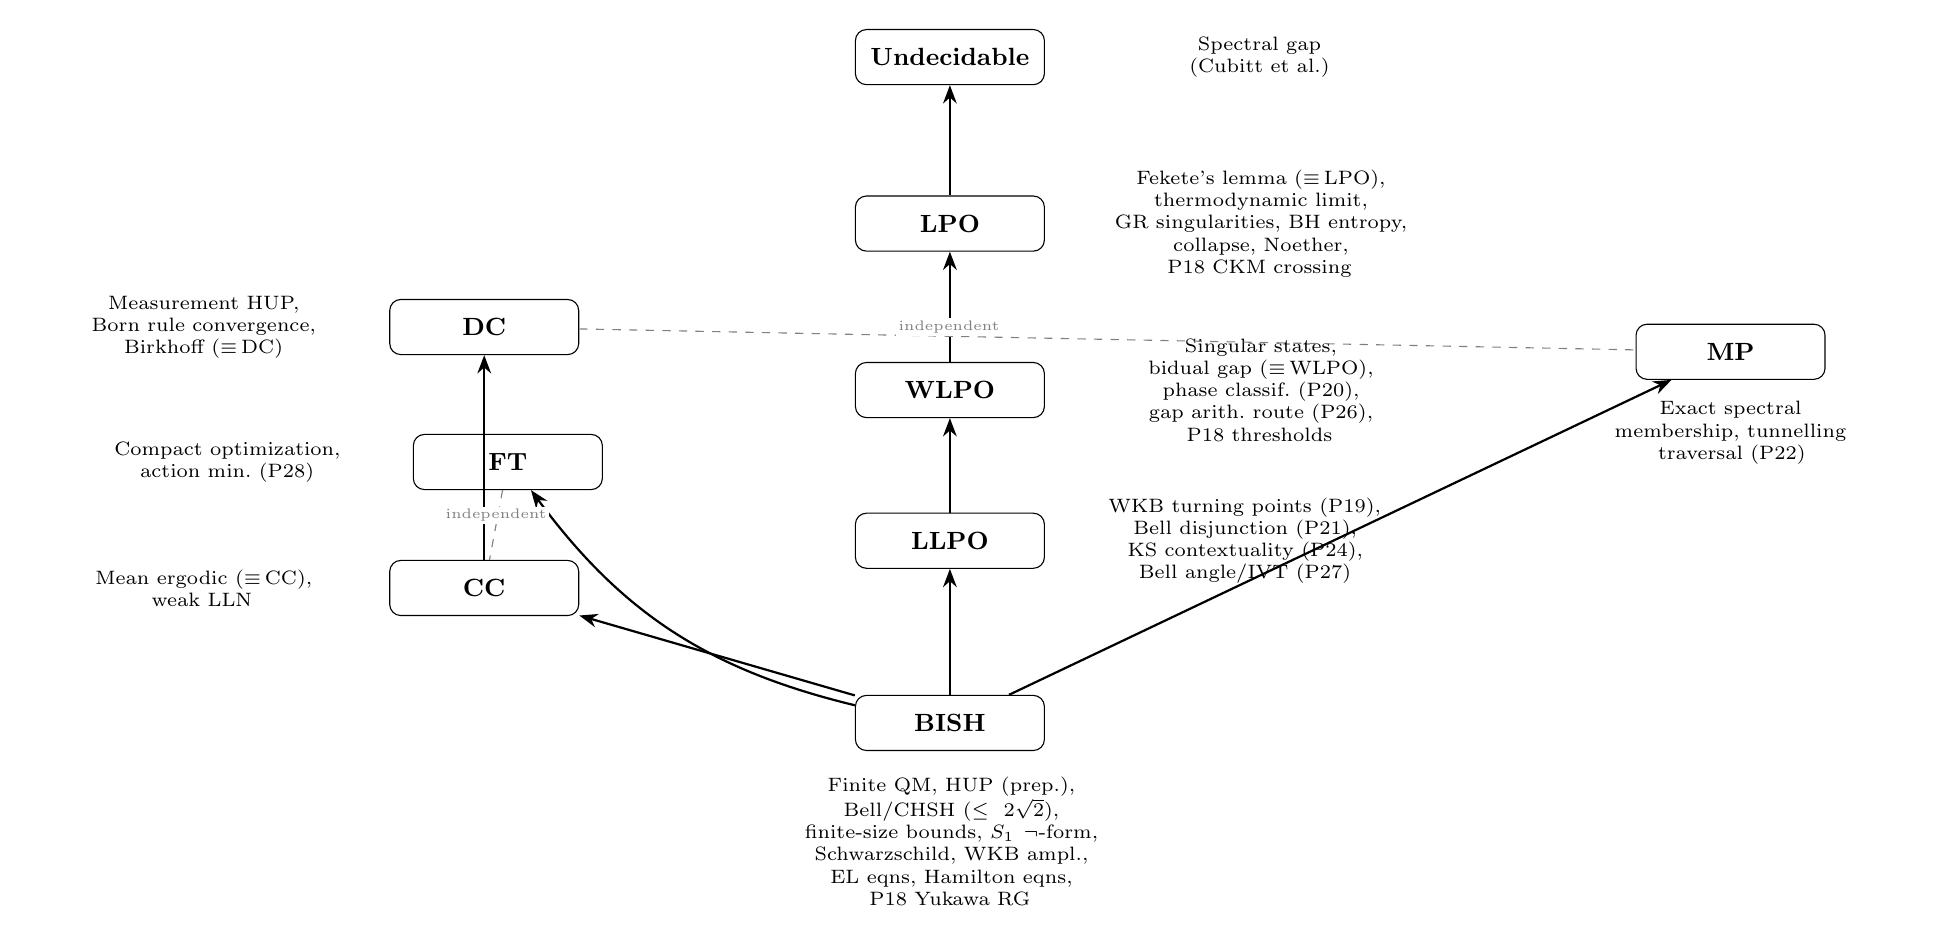
\begin{tikzpicture}[
  node distance=1.4cm and 2.8cm,
  principle/.style={draw, rounded corners, minimum width=2.4cm, minimum height=0.7cm, font=\small\bfseries},
  physlabel/.style={font=\scriptsize, text width=4.2cm, align=center},
  >=Stealth
]
% Main spine
\node[principle] (bish) {BISH};
\node[principle, above=1.6cm of bish] (llpo) {LLPO};
\node[principle, above=1.2cm of llpo] (wlpo) {WLPO};
\node[principle, above=of wlpo] (lpo) {LPO};
\node[principle, above=of lpo] (undec) {Undecidable};

% Choice hierarchy (refined: CC < DC) — DC between WLPO and LPO, far left
\node[principle, above left=1.0cm and 3.5cm of bish] (cc) {CC};
\node[principle, above=2.6cm of cc] (dc) {DC};
% Orthogonal branches — MP between WLPO and LPO so DC--MP line clears WLPO labels
\node[principle, above right=4.0cm and 7.5cm of bish] (mp) {MP};
\node[principle, below left=0.2cm and 3.2cm of wlpo] (ft) {FT};

% Edges (Hasse diagram: only covering relations)
\draw[thick, ->] (bish) -- (cc);
\draw[thick, ->] (cc) -- (dc);
\draw[thick, ->] (bish) -- (mp);
\draw[thick, ->] (bish) -- (llpo);
\draw[thick, ->] (llpo) -- (wlpo);
\draw[thick, ->] (wlpo) -- (lpo);
\draw[thick, ->] (lpo) -- (undec);
\draw[thick, ->] (bish) to[bend left=20] (ft);

% Physical labels
\node[physlabel, below=0.2cm of bish] {Finite QM, HUP (prep.),\\Bell/CHSH ($\leq 2\sqrt{2}$),\\finite-size bounds, $S_1\;\neg$-form,\\Schwarzschild, WKB ampl.,\\EL eqns, Hamilton eqns,\\P18 Yukawa RG};
\node[physlabel, left=0.15cm of cc] {Mean ergodic ($\equiv$\,CC),\\weak LLN};
\node[physlabel, left=0.15cm of dc] {Measurement HUP,\\Born rule convergence,\\Birkhoff ($\equiv$\,DC)};
\node[physlabel, below=0.15cm of mp] {Exact spectral\\membership, tunnelling\\traversal (P22)};
\node[physlabel, left=0.15cm of ft] {Compact optimization,\\action min.\ (P28)};
\node[physlabel, right=0.5cm of llpo, text width=3.8cm] {WKB turning points (P19),\\Bell disjunction (P21),\\KS contextuality (P24),\\Bell angle/IVT (P27)};
\node[physlabel, right=0.5cm of wlpo] {Singular states,\\bidual gap ($\equiv$\,WLPO),\\phase classif.\ (P20),\\gap arith.\ route (P26),\\P18 thresholds};
\node[physlabel, right=0.5cm of lpo] {Fekete's lemma ($\equiv$\,LPO),\\thermodynamic limit,\\GR singularities, BH entropy,\\collapse, Noether,\\P18 CKM crossing};
\node[physlabel, right=0.5cm of undec] {Spectral gap\\(Cubitt et al.)};

% Orthogonality annotations (fill=white, pos shifted to avoid label overlap)
\draw[dashed, gray] (dc) -- node[above, font=\tiny, gray, fill=white, inner sep=1pt, pos=0.35] {independent} (mp);
\draw[dashed, gray] (ft) -- node[above, font=\tiny, gray, fill=white, inner sep=1pt] {independent} (cc);

\end{tikzpicture}%
}% end resizebox
\caption{The logical geography of mathematical physics: a Hasse diagram (v5.0).
Arrows indicate strict implication over BISH\@. The omniscience spine
(BISH $<$ LLPO $<$ WLPO $<$ LPO) forms the dominant vertical chain. CC $<$ DC, MP, and FT
occupy orthogonal positions: none implies any other, and none implies WLPO.
Physical layers are annotated with their calibrated logical cost from Papers~2--28.
All entries are machine-verified; ``$\equiv$'' denotes proven equivalence over BISH.}
\label{fig:hasse}
\end{figure}

The calibration table is displayed in Figure~\ref{fig:hasse}.
Return to the mountain metaphor.

\textbf{Sea level (BISH).}
Everything a laboratory does lives here: finite quantum mechanics, preparation uncertainty~\eqref{eq:rs-inequality}, Bell nonlocality~\eqref{eq:chsh}, entanglement entropy, finite-size Ising bounds~\eqref{eq:ising-bound}, local general relativity including the Raychaudhuri equation~\eqref{eq:raychaudhuri} and the Schwarzschild vacuum, Euler-Lagrange and Hamilton's equations (Paper~28), and the Yukawa RG one-loop flow (Paper~18; the same paper's Lean formalization shows threshold decoupling costs WLPO and CKM eigenvalue-crossing detection costs LPO). No omniscience principle or appeal to the law of excluded middle is needed for the core computations.

\textbf{The foothills (CC, DC, MP, FT).}
Paper~25 \cite{Lee2026paper25} sharpens the choice axis: ensemble convergence (mean ergodic theorem, weak LLN) requires only Countable Choice; individual-trajectory convergence (Birkhoff, strong LLN) requires the stronger Dependent Choice. Measurement uncertainty \cite{Lee2026g} and the measurement problem (Paper~16) are DC phenomena. Exact spectral membership requires Markov's Principle \cite{Lee2026f}; the tunnelling traversal time controversy (Paper~22) is an MP disagreement. The Fan Theorem---asserting that a continuous function on a compact set attains its minimum---requires FT \cite{Lee2026paper23}, independent of the entire omniscience spine; classical mechanics variational principles (Paper~28) provide a second FT calibration. These branches are mutually independent.

\textbf{The LLPO ledge.}
Four calibrations populate the level between BISH and WLPO: WKB turning-point existence \cite{Lee2026paper19}, Bell's disjunction \cite{Lee2026paper21}, KS contextuality \cite{Lee2026paper24}, and Bell angle optimization via the IVT \cite{Lee2026paper27}. All share the structure of disjunction without constructive witness.

\textbf{The mountainside (WLPO).}
Singular states in the bidual \cite{Lee2026a, Lee2026b}, phase classification of the Ising model \cite{Lee2026paper20}, and bidual gap detection via an independent arithmetic route \cite{Lee2026paper26} all cost exactly WLPO\@.

\textbf{The summit (LPO).}
The thermodynamic limit is equivalent to LPO \cite{Lee2026c}, verified across two independent formulations \cite{Lee2026e}. The same BMC~$\equiv$~LPO equivalence governs geodesic incompleteness \cite{Lee2026paper13}, exact decoherence \cite{Lee2026paper14}, global energy conservation \cite{Lee2026paper15}, and BH entropy convergence \cite{Lee2026paper17}---five independent domains, one abstract principle.

\textbf{Beyond the summit (undecidable).}
The spectral gap problem \cite{Cubitt2015} is undecidable in the Turing sense---orthogonal to the logical-strength hierarchy. For any finite lattice the spectral gap is BISH-computable; undecidability enters through the thermodynamic limit, the same limit that costs LPO\@. The two hierarchies are distinct but agree on where the physics--formalism boundary falls: finite systems are BISH/decidable; infinite idealizations sit above BISH in both.

Two features of this table deserve emphasis.

First, \emph{formulation-invariance}.
The LPO cost of the thermodynamic limit was derived independently via two completely different mathematical routes: a transfer-matrix method using eigenvalue analysis and linear algebra, and a purely combinatorial method using bond variables and a binomial parity sieve with no matrices or functional analysis \cite{Lee2026e}.
The axiom profiles are identical.
This is evidence that the logical cost is a property of the physics, not of the mathematician's choice of formalism.

Second, \emph{machine verification}.
These results are not informal arguments about what ``should'' be constructive.
They are Lean~4 proof terms, machine-checked end-to-end, with \texttt{\#print axioms} certificates that list every non-constructive axiom used in each proof.
The total is approximately 24,500~lines of formally verified code.
The proof assistant enforces logical bookkeeping at a scale that no informal method could sustain across 23{,}000~lines: it ensures that no classical axiom sneaks in through a library import, a typeclass resolution, or an unnoticed appeal to decidability.


% ============================================================
\section{What Could Have Been Done Instead}
\label{sec:alternatives}
% ============================================================

The calibration table is not merely a diagnosis; it suggests a therapy.
The remarkable fact is that physicists \emph{already compute at BISH}---a fact implicit in computational practice but not previously made explicit.
The constructive alternatives to the classical formalism are not radical proposals for a new physics.
They are descriptions of what physicists actually do: finite-size error bounds instead of the thermodynamic limit~\eqref{eq:ising-bound}, the Cauchy-Schwarz inequality instead of spectral theory for uncertainty~\eqref{eq:rs-inequality}, finite-dimensional linear algebra for Bell nonlocality~\eqref{eq:chsh}, finite-parameter differential equations for gravitational focusing~\eqref{eq:raychaudhuri}, and finite-order Feynman diagrams instead of path integrals.
In every case the constructive alternative is what the working physicist is already doing.
The formalism merely pretends otherwise.

Moreover, several post-war developments are themselves constructive frameworks, often unrecognized as such:
Wilson's lattice gauge theory (1974) \cite{Wilson1974} computes hadron masses on finite grids at BISH;
effective field theory (Weinberg, 1979+) keeps calculations at finite loop order without claiming convergence;
tensor network methods (White 1992, Vidal 2003+) provide finite-dimensional variational approaches avoiding infinite-dimensional Hilbert spaces;
validated numerics produces rigorous finite-precision bounds via interval arithmetic.
The constructive alternative is not hypothetical; it is how much of computational physics already operates.
Our programme (2026) adds the logical anatomy: Bell nonlocality at BISH, measurement at DC$_\omega$, tunnelling at MP, WKB turning points at LLPO, variational principles at FT---separating physical content from formalism at every level.

\begin{figure}[ht]
\centering
\resizebox{\textwidth}{!}{%
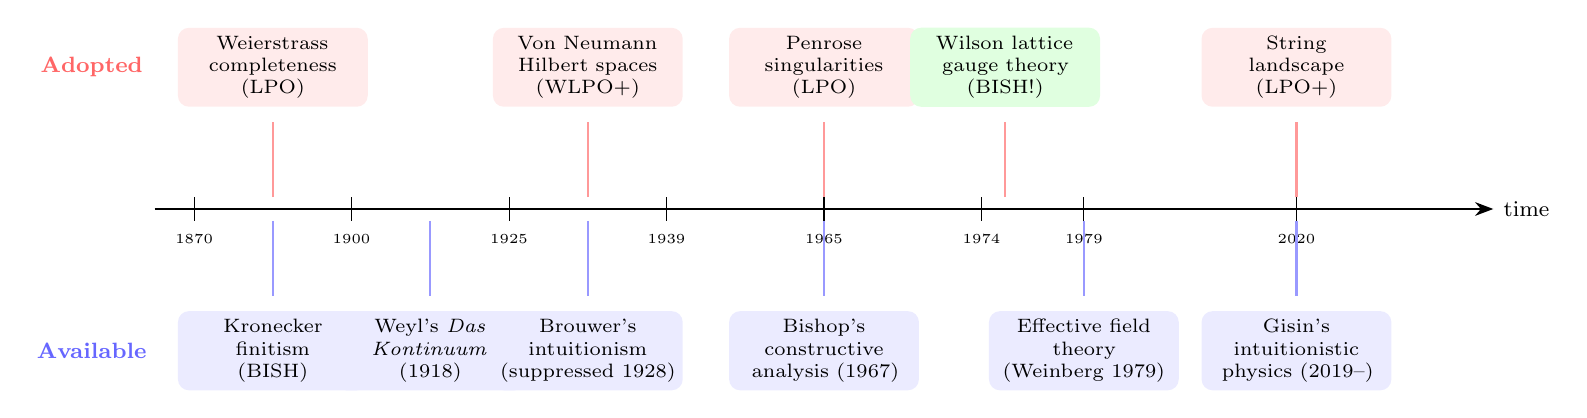
\begin{tikzpicture}[
  >=Stealth,
  every node/.style={font=\scriptsize},
  event/.style={circle, fill, inner sep=1.5pt},
  adopted/.style={font=\scriptsize, text width=2.2cm, align=center, fill=red!8, rounded corners, inner sep=3pt},
  alternative/.style={font=\scriptsize, text width=2.2cm, align=center, fill=blue!8, rounded corners, inner sep=3pt}
]
% Timeline
\draw[thick, ->] (0,0) -- (17, 0) node[right] {\footnotesize time};
% Tick marks
\foreach \x/\y in {0.5/1870, 2.5/1900, 4.5/1925, 6.5/1939, 8.5/1965, 10.5/1974, 11.8/1979, 14.5/2020} {
  \draw (\x, -0.15) -- (\x, 0.15);
  \node[below, font=\tiny] at (\x, -0.2) {\y};
}
% Upper track: what was adopted (red-tinted)
\node[adopted] at (1.5, 1.8) {Weierstrass\\completeness\\(LPO)};
\node[adopted] at (5.5, 1.8) {Von Neumann\\Hilbert spaces\\(WLPO+)};
\node[adopted] at (8.5, 1.8) {Penrose\\singularities\\(LPO)};
\node[adopted, fill=green!12] at (10.8, 1.8) {Wilson lattice\\gauge theory\\(BISH!)};
\node[adopted] at (14.5, 1.8) {String\\landscape\\(LPO+)};
% Lower track: what was available (blue-tinted)
\node[alternative] at (1.5, -1.8) {Kronecker\\finitism\\(BISH)};
\node[alternative] at (3.5, -1.8) {Weyl's \emph{Das\\Kontinuum}\\(1918)};
\node[alternative] at (5.5, -1.8) {Brouwer's\\intuitionism\\(suppressed 1928)};
\node[alternative] at (8.5, -1.8) {Bishop's\\constructive\\analysis (1967)};
\node[alternative] at (11.8, -1.8) {Effective field\\theory\\(Weinberg 1979)};
\node[alternative] at (14.5, -1.8) {Gisin's\\intuitionistic\\physics (2019--)};
% Arrows connecting to timeline
\foreach \x in {1.5, 5.5, 8.5, 10.8, 14.5} {
  \draw[red!40, thick] (\x, 0.15) -- (\x, 1.1);
}
\foreach \x in {1.5, 3.5, 5.5, 8.5, 11.8, 14.5} {
  \draw[blue!40, thick] (\x, -0.15) -- (\x, -1.1);
}
% Labels for tracks
\node[font=\footnotesize\bfseries, red!60] at (-0.8, 1.8) {Adopted};
\node[font=\footnotesize\bfseries, blue!60] at (-0.8, -1.8) {Available};
\end{tikzpicture}%
}% end resizebox
\caption{The road not taken. At every stage where classical logic was imported into
physics (upper track, red), a constructive alternative was available (lower track, blue).
Wilson's lattice gauge theory (green, 1974) is the exception: an adopted framework
that is itself BISH\@.
The constructive road was not taken---not because it was mathematically inadequate,
but because the classical road was more convenient and its logical cost was invisible.
Paper~29 reveals a limitation: for generic systems near phase transitions, no constructive road exists---Fekete's lemma ($\equiv$ LPO) is the only route. The road not taken was available for tiers~1--2; for tier~3, the classical road was the only road.}
\label{fig:timeline}
\end{figure}


\subsection*{The cognitive value of idealization}

If the constructive alternative suffices for every prediction, a natural objection arises: why did every great physicist of the twentieth century use the cathedral?
Einstein was not confused.
Von~Neumann was not following convention.
Dirac was not ignorant of alternatives.
They chose the idealizations because the idealizations let them \emph{think}.

Consider the path to general relativity.
Einstein's 1915 field equations $G_{\mu\nu} = 8\pi T_{\mu\nu}$ are a finite system of PDEs relating finite objects---metric components, their derivatives, stress-energy.
Writing them down requires no idealization; the route to them through differential geometry and tensor calculus is algebraic and BISH\@.
But Einstein arrived at these equations by thinking of spacetime as a smooth manifold, gravity as curvature, geodesics as paths of free particles.
That geometric picture, while not formally requiring non-constructive logic, is deeply entangled with the idea of a completed continuum---a smooth, infinite, everywhere-defined mathematical object.
The picture guided ten years of creative struggle (1905--1915).

Once the equations were written, every empirical prediction Einstein extracted was BISH\@.
The perihelion precession of Mercury: a perturbative solution of the geodesic equation in the Schwarzschild metric, yielding $\delta\varphi = 6\pi GM/(c^2 a(1-e^2))$.
Finite computation, algebraic result.
Gravitational redshift: $\nu_2/\nu_1 = \sqrt{g_{00}(r_1)/g_{00}(r_2)}$.
One formula, one substitution.
Gravitational lensing: $\delta = 4GM/(c^2 b)$.
A definite integral with an explicit integrand.
Every number Einstein compared with observation was a BISH computation from specific equations evaluated at specific parameters.

The same pattern holds for quantum mechanics.
Heisenberg's 1925 matrix mechanics was explicitly finite and algebraic---transition amplitudes as finite matrix elements, the hydrogen spectrum by finite matrix truncation.
This is BISH\@.
Schr\"odinger's 1926 wave mechanics introduced the wave function $\psi(x) \in L^2(\mathbb{R}^3)$---an infinite-dimensional Hilbert space---but every calculation Schr\"odinger actually performed reduced to solving a specific differential equation with specific boundary conditions.
The hydrogen eigenvalue $E_n = -13.6/n^2$~eV comes from a boundary-value problem for a second-order ODE; each specific eigenvalue is computable by algebraic manipulation.
No spectral theorem is invoked.
The spectral theorem enters when you assert that these are \emph{all} the eigenvalues and that the eigenfunctions form a \emph{complete} basis---an assertion about a completed infinite object that organizes the physics but generates no additional predictions.

The idealizations serve as \emph{cognitive infrastructure}: they convert processes into objects.
The thermodynamic limit converts an open-ended approximation (``the free energy per site is within~$\varepsilon$ of $f(\beta)$ for lattice size $N(\varepsilon)$'') into a definite fact (``the free energy is $f(\beta)$'').
The first is a bound you can compute with.
The second is a thought you can compose with other thoughts---you can differentiate it, take its Legendre transform, study its singularities.
The spectral theorem converts an open-ended list (``these specific eigenvalues satisfy these specific equations'') into a completed structure (``every self-adjoint operator has a spectral decomposition'').
The first handles specific systems.
The second enables general theory---perturbation theory, scattering theory, the classification of quantum symmetries.
Each idealization converts a BISH computation into a mathematical object that can be manipulated, composed, and reasoned about at a higher level of abstraction.
The logical cost, measured by the calibration table, is the price of that conversion.

The calibration table, read through this lens, becomes a cost-benefit analysis of idealization.
Not all idealizations are equal.
The thermodynamic limit (LPO) converts approximation processes into definite thermodynamic potentials, enabling all of equilibrium statistical mechanics---phase transitions, critical exponents, universality.
High cognitive return on the logical investment.
The Penrose singularity (LPO) converts finite-time geodesic focusing into a definite incompleteness theorem, enabling the entire programme of black hole physics.
High cognitive return.
The singular states of the bidual (WLPO) produce a mathematical object---a functional that vanishes on all compact operators---that no experiment can prepare and no physical reasoning builds upon.
Low cognitive return.
The calibration table provides the cost side of this ledger; the history of physics provides the benefit side.
Together, they distinguish productive idealizations from pathological ones---not by taste, but by measurement.

The engineering confirms this assessment.
Every technology based on twentieth-century physics---GPS, semiconductors, lasers, MRI, nuclear energy---uses specific finite computations at BISH\@.
The relativistic corrections in GPS (${\sim}38$~microseconds per day, compensating the net effect of special-relativistic time dilation and general-relativistic gravitational blueshift) are arithmetic: one algebraic formula from the Schwarzschild metric evaluated at the satellite's orbital parameters.
The atomic clock frequency (cesium-133 hyperfine transition at 9,192,631,770~Hz) is computed from specific quantum-mechanical matrix elements.
No spectral theorem, no completed Hilbert space, no thermodynamic limit appears in any engineering specification.
The cathedral guides the theorist's thinking.
The cellar runs the devices.

\bigskip

\textbf{The programme's trajectory.} Before stating the thesis, it is worth noting that the programme passed through four phases---from early probes (Papers~2--7) through the BMC~$\equiv$~LPO paradigm (Papers~8--15) and frontier tests (Papers~16--18) to the complete tree (Papers~19--28). The full development is traced in Appendix~\ref{app:development}.

% ============================================================
\section{The Grand Thesis}
\label{sec:thesis}
% ============================================================

We are now in a position to state the working hypothesis of the research programme.

\textbf{The hypothesis, refined}: the correlation between constructive logical strength and degree of physical idealization is not accidental.
For every exactly solvable model and every system with explicit finite-size bounds examined so far, empirical predictions---the outputs of physical theory for finite experimental specifications---are BISH-derivable.
Stronger logical principles enter through idealizations that no finite laboratory can instantiate, and the hierarchy of those principles is a tree, not a chain: the omniscience spine (BISH $<$ LLPO $<$ WLPO $<$ LPO), with independent branches for the choice hierarchy (CC $<$ DC, refined by Paper~25), MP, and FT.
Moreover, the logical cost is \emph{observable-dependent}: the same physical system (e.g., the 1D Ising model) can cost LPO for one question (the thermodynamic limit, Paper~8) and only WLPO for another (phase classification, Paper~20).

But Paper~29 \cite{Lee2026paper29Fekete} compels a qualification that transforms the hypothesis.
Fekete's Subadditive Lemma---every subadditive sequence with $u_n/n$ bounded below converges---is equivalent to LPO over BISH\@.
Since the thermodynamic limit proceeds via subadditivity of the log-partition function, the LPO cost is ineliminable for any system that lacks an explicit closed-form or cluster-expansion modulus.
Near phase transitions, where correlation lengths diverge and all explicit bounds fail, there is no BISH alternative.
The cellar handles tiers~1 and~2; tier~3 belongs to the cathedral.

If the original pattern held without exception, nature would operate at BISH, and classical mathematics would be the mathematician's convenience, not nature's requirement.
Paper~29 shows the reality is more interesting: nature operates at BISH for every prediction we can extract from specific, tractable models, but the mathematical description of generic critical phenomena requires LPO ineliminably.
The universe may not be a Turing machine.

This hypothesis is not operationalism.
Operationalism says: only observable quantities are meaningful.
Our hypothesis says something more precise: the logical principles needed to derive observable quantities are strictly weaker than the principles assumed by the standard formalism.
The thermodynamic limit is not ``meaningless''---it is mathematically well-defined, and it provides a useful computational shortcut.
But its logical cost is LPO, and the empirical predictions it delivers are available at BISH.
The hypothesis distinguishes the \emph{physical content} of a formalism (which lives at BISH) from its \emph{mathematical infrastructure} (which may require WLPO, LPO, or more).

There is a historical parallel that illuminates the thesis without overstating it.
When Einstein formulated special relativity in 1905, his key insight was that absolute simultaneity---a structural feature of Newtonian mechanics that no experiment could detect---was surplus.
Removing it was not a loss but a clarification: the physics was already there; the surplus structure was obscuring it.
Our hypothesis suggests an analogous move applied to the logical infrastructure of mathematics itself.
The non-constructive superstructure of classical analysis is surplus structure for tiers~1 and~2---exactly solvable models and cluster expansions.
But Paper~29 shows it is not surplus for tier~3: Fekete's lemma is equivalent to LPO, and for generic systems near criticality, no weaker principle suffices.
The analogy with special relativity holds partially: some classical structure is surplus (like absolute simultaneity), but other structure (like the Lorentz group itself) is indispensable.
The calibration table distinguishes the surplus from the indispensable.
If this refined analogy holds, 150~years of mathematical physics have progressively imported logical strength---omniscience for limits, choice for ergodic theory, compactness for variational principles---while the empirical content remained BISH for specific, tractable models.
For the generic case near phase transitions, the non-constructive superstructure is not the mapmaker's convention; it may be the territory.

The relationship between BISH and the Church-Turing thesis is more subtle than the original hypothesis suggested.
For tiers~1 and~2, every empirical prediction is BISH-derivable, and the Church-Turing thesis holds \emph{a fortiori}: every physically realizable computation is Turing-computable.
But tier~3---generic systems near criticality---requires LPO, which transcends what any Turing machine can decide in finite time.
The universe, at the level of its mathematical description near phase transitions, may not be a Turing machine.
This is not a speculative extrapolation; it is a theorem: Fekete's lemma is equivalent to LPO, and Fekete's lemma is the tool that extracts the thermodynamic limit from subadditivity.
If the physical universe undergoes genuine phase transitions described by the mathematical framework of statistical mechanics, then LPO is doing real physical work---the cathedral is not idle.
The hypothesis occupies a specific position between bare computability and full classical logic---but the position is more nuanced than ``nature is computable'': nature is computable where we can compute explicitly (tiers~1--2), and it requires omniscience where we cannot (tier~3).

The closest philosophical predecessor is Gisin \cite{Gisin2020, Gisin2021}, who argues that real numbers contain infinite information, that finite physical systems cannot, and therefore that intuitionistic mathematics is the natural language for physics.
Our programme supplies the formal precision that Gisin's vision lacks.
Where Gisin says ``something like BISH,'' we provide a calibration table that distinguishes BISH from WLPO from LPO, backed by machine-verified proofs.
Gisin provides the philosophical motivation; our programme provides the mathematical evidence.

But the programme's results are now precise enough to adjudicate three major positions in the philosophy of mathematics and computation---not merely to acknowledge them as predecessors, but to measure their claims against the calibration table.

\emph{Brouwer.} Brouwer's core thesis---that classical logic is illegitimate for reasoning about infinite objects---is partially vindicated and partially refuted.
He was right that the infinite costs something: the calibration table is a precise accounting of \emph{what} it costs.
Every completed infinite object in physics (thermodynamic limit, geodesic completion, exact decoherence) pays LPO, exactly as Brouwer's intuition would predict.
His emphasis on compactness as a distinct logical resource is vindicated by the Fan Theorem's independence: Papers~23 and~28 show that variational reasoning draws on a well (FT) entirely separate from convergence reasoning (LPO).
But Brouwer rejected classical mathematics \emph{entirely}---as philosophically illegitimate, not merely unnecessary.
The programme shows classical mathematics is not illegitimate; it is \emph{expensive}.
For tiers~1 and~2, the expense is unnecessary (all predictions are available at BISH).
For tier~3, Fekete~$\equiv$~LPO shows the expense is unavoidable: Brouwer would have rejected the only mathematics that can describe generic phase transitions.
His intuition was sound; his prohibition was too strong.

\emph{Bishop.} Bishop's constructive analysis \cite{Bishop1967}---the claim that BISH suffices for all meaningful mathematics, and that the classical superstructure is ``a scandal''---is the programme's most direct predecessor.
For tiers~1 and~2, Bishop was remarkably right: every empirical prediction from every specific tractable model we have examined is BISH-derivable.
Bishop's constructive analysis \emph{is} the cellar.
The most precise prediction in physics (the electron $g{-}2$ factor, twelve decimal places) requires nothing beyond Bishop's framework.
But Paper~29 shows Bishop went too far.
Fekete~$\equiv$~LPO means that for generic systems near criticality---where correlation lengths diverge and all explicit bounds fail---there is no BISH alternative.
The thermodynamic limit for systems without explicit convergence moduli \emph{requires} LPO\@.
Bishop might respond that non-computable limits are not meaningful mathematics; the programme responds that if nature undergoes genuine phase transitions, the mathematics that describes them is meaningful whether or not it is computable.
The cathedral is sometimes more than convenience.

\emph{Wolfram and digital physics.} The strongest computational claim---Wolfram's thesis \cite{Wolfram2002} that the universe \emph{is} a computation, reducible to simple rules iterated on a discrete substrate---receives the sharpest refutation.
If the universe were a cellular automaton or a Turing machine, every physical phenomenon should be describable at BISH or below.
For tiers~1 and~2, the digital physics vision is consistent: every specific prediction is a finite computation, and the cellar is a Turing machine.
But tier~3 flatly contradicts it.
Fekete's lemma is the only route to the generic thermodynamic limit, and Fekete~$\equiv$~LPO, which transcends what any Turing machine can decide in finite time.
This is not a philosophical argument; it is a theorem.
If the physical universe undergoes genuine phase transitions described by the mathematical framework of statistical mechanics, then its mathematical description requires a principle no algorithm can implement.
The digital physics programme must either explain how phase transitions work without Fekete's lemma---and the programme shows no such explanation exists---or accept that the universe, at the level of mathematical description, is not a Turing machine.

\emph{Implications for relativity.} The programme's results split general relativity along the BISH/LPO boundary with striking precision.
Local physics---curvature at finite radius (Paper~5), the Schwarzschild interior's finite-time trajectories (Paper~13), the relativistic corrections in GPS (algebraic evaluation of the Schwarzschild metric at specific orbital parameters)---is entirely BISH\@.
A GPS satellite is a BISH machine.
Global completions---geodesic incompleteness (Paper~13), singularity theorems, the assertion that infalling worldlines \emph{terminate}---cost LPO via BMC\@.
The local/global split that general relativists have long recognized as physically fundamental coincides exactly with the BISH/LPO boundary.
The event horizon is not merely a physical boundary; it is a logical boundary (Paper~13).

\emph{Implications for quantum physics.} Quantum mechanics splits even more cleanly.
The algebraic structure that makes quantum physics ``strange''---uncertainty relations (Paper~6), Bell violations (Paper~11), the Tsirelson bound (Paper~11), entanglement entropy (Paper~11), Born probabilities (Paper~16), Kochen-Specker uncolorability (Paper~24)---is entirely BISH\@.
The spookiness of quantum mechanics is computationally innocent.
The disjunctive conclusions that physicists draw from no-go theorems---``either locality fails \emph{or} realism fails'' (Paper~21), ``either non-contextuality fails \emph{or} value-definiteness fails'' (Paper~24)---cost LLPO: the refutation is free, the disjunction is not.
The infinite limits that generate interpretive controversy---exact decoherence (Paper~14), the measurement problem's frequentist convergence (Paper~16)---cost LPO and DC$_\omega$ respectively.
The implication is pointed: the interpretive controversies of quantum foundations---Copenhagen versus many-worlds versus Bohmian mechanics---may be, in part, disagreements about which logical principles to accept for infinite limits, not disagreements about the finite physics.
The finite quantum mechanics is both uncontroversial and constructive; the controversy lives in the cathedral.

\begin{center}
\begin{tabular}{@{}lccc@{}}
\toprule
 & \textbf{Tiers 1--2} & \textbf{Tier 3} & \textbf{Overall} \\
\midrule
Brouwer: classical logic fails & Vindicated & Refuted & Partially right \\
Bishop: BISH suffices & Vindicated & Refuted & Partially right \\
Wolfram: universe is a computation & Consistent & Refuted & Refuted \\
\bottomrule
\end{tabular}
\end{center}

\noindent All three positions capture something real about tiers~1 and~2---the cellar \emph{is} constructive, \emph{is} computable, and \emph{does} suffice for empirical prediction.
All three fail at tier~3, where the programme's results show the non-constructive superstructure is not idle but ineliminable.
The calibration table adjudicates with a precision that philosophical argument alone cannot achieve.

A refinement of the hypothesis, visible only since Papers~19--25, deserves emphasis: the logical cost depends on the \emph{observable}, not merely the \emph{system}.
The 1D Ising model costs LPO for the thermodynamic limit but only WLPO for phase classification.
Quantum tunnelling is BISH for a specific barrier but LLPO for turning-point existence in a general potential.
Bell's theorem is BISH for the violation bound but LLPO for the disjunction.
This observable-dependence is a finer-grained structure than domain invariance; it shows that the constructive hierarchy measures the logical cost of the \emph{question asked of nature}, not merely the system under study.

Why should this pattern demand explanation?
The correlation is not between logical strength and mathematical generality---simple theorems can be non-constructive (the thermodynamic limit is just a limit of a monotone sequence), and complex theorems can be constructive (the Ising error bounds involve transfer matrices, eigenvalues, and geometric series analysis).
The correlation is between logical strength and \emph{physical idealization}: whether a finite laboratory can instantiate the objects described.
Five phenomena, taken together, point beyond calibration toward something deeper.
\emph{Domain invariance}: BMC~$\equiv$~LPO governs completed limits in five unrelated domains---not because they share mathematics, but because they share the operation of infinite completion.
\emph{Structural identity}: Bell and KS share LLPO cost for structural reasons, not coincidence---the proof assistant reveals a kinship invisible to informal analysis.
\emph{Diagnostic power}: CRM resolves genuine physical controversies---the tunnelling traversal time debate is an MP disagreement (Paper~22); part of the measurement problem is a DC$_\omega$ disagreement (Paper~16).
\emph{Observable-dependence}: the same system has different costs for different questions.
\emph{Choice-axis refinement}: ensemble convergence and individual convergence draw on different levels of the same axis (Paper~25).
If five independent phenomena all point the same way, the pattern is unlikely to be an artifact of how we chose to formalize.

The hypothesis suggests a principle---not yet proven, but gestured at by the evidence---that might serve as a foundation: \emph{the empirical content of a physical theory is invariant under replacement of its mathematical formalism by any other formalism that produces the same finite-precision predictions.}
This is a logical equivalence principle: any two formalisms that agree at BISH are physically equivalent, regardless of what they assert at WLPO, LPO, or LEM.
The calibration table then becomes a diagnostic tool for identifying which parts of a formalism are doing physical work and which are idle mathematical machinery.

\begin{figure}[ht]
\centering
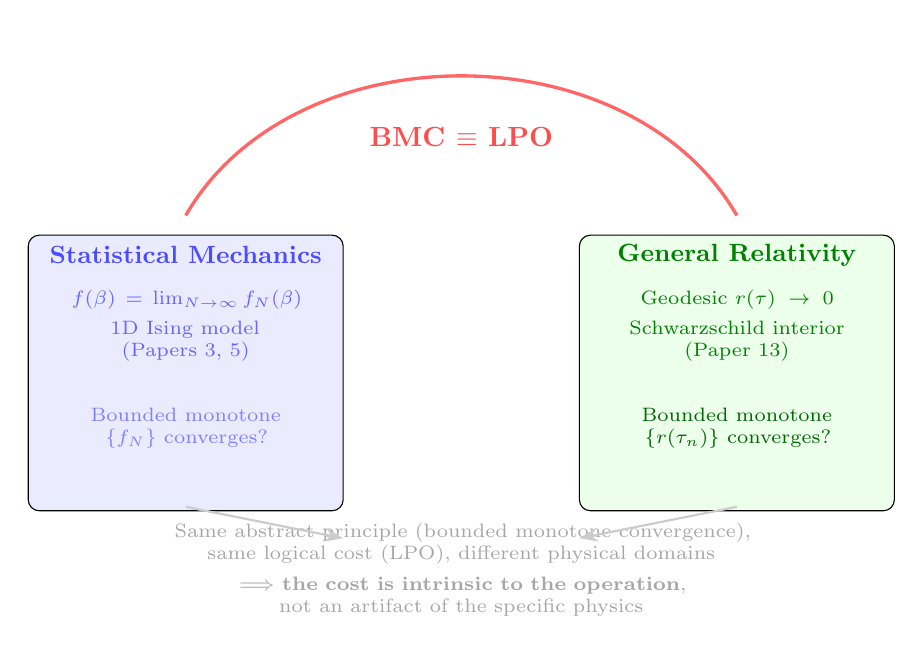
\begin{tikzpicture}[
  >=Stealth,
  every node/.style={font=\small},
  pillar/.style={draw, rounded corners, minimum width=4cm, minimum height=3.5cm, align=center, inner sep=6pt}
]
% Left pillar: Statistical Mechanics
\node[pillar, fill=blue!8] (sm) at (-3.5, 0) {};
\node[font=\small\bfseries, blue!70] at (-3.5, 1.5) {Statistical Mechanics};
\node[font=\scriptsize, blue!60, text width=3.5cm, align=center] at (-3.5, 0.6)
  {$f(\beta) = \lim_{N\to\infty} f_N(\beta)$\\[3pt]1D Ising model\\(Papers 3, 5)};
\node[font=\scriptsize, blue!50, text width=3.5cm, align=center] at (-3.5, -0.7)
  {Bounded monotone\\$\{f_N\}$ converges?};

% Right pillar: General Relativity
\node[pillar, fill=green!8] (gr) at (3.5, 0) {};
\node[font=\small\bfseries, green!50!black] at (3.5, 1.5) {General Relativity};
\node[font=\scriptsize, green!50!black, text width=3.5cm, align=center] at (3.5, 0.6)
  {Geodesic $r(\tau) \to 0$\\[3pt]Schwarzschild interior\\(Paper 13)};
\node[font=\scriptsize, green!40!black, text width=3.5cm, align=center] at (3.5, -0.7)
  {Bounded monotone\\$\{r(\tau_n)\}$ converges?};

% Bridge/arch
\draw[very thick, red!60] (-3.5, 2.0) to[out=60, in=120] (3.5, 2.0);
\node[font=\normalsize\bfseries, red!70, fill=white, inner sep=3pt] at (0, 3.0)
  {BMC $\equiv$ LPO};

% Below: explanation
\node[font=\scriptsize, gray!70, text width=8cm, align=center] at (0, -2.5)
  {Same abstract principle (bounded monotone convergence),\\
   same logical cost (LPO), different physical domains\\[3pt]
   $\Longrightarrow$ \textbf{the cost is intrinsic to the operation},\\
   not an artifact of the specific physics};

% Arrows down to explanation
\draw[->, thick, gray!40] (-3.5, -1.7) -- (-1.5, -2.1);
\draw[->, thick, gray!40] (3.5, -1.7) -- (1.5, -2.1);

\end{tikzpicture}
\caption{Domain invariance: the same logical cost in different physics.
The bounded monotone convergence equivalence (BMC~$\equiv$~LPO) appears
independently in statistical mechanics (thermodynamic limit) and general
relativity (geodesic incompleteness).
That the same abstract principle governs both is evidence that the logical
cost is intrinsic to the mathematical operation, not to the physical domain.
Paper~29 identifies the mechanism: Fekete's Subadditive Lemma ($\equiv$ LPO) is the generic tool for extracting limits from subadditivity.}
\label{fig:domain-invariance}
\end{figure}

\begin{keymessage}
\textbf{Hypothesis:} empirical predictions are BISH-derivable; stronger logic enters only through idealizations no finite laboratory can instantiate.
This is not operationalism---it distinguishes physical content (BISH) from mathematical infrastructure (WLPO/LPO/LEM).
For tiers~1 and~2, the non-constructive superstructure is physically idle.
For tier~3 (generic systems near criticality), Paper~29 shows it is ineliminable.
\end{keymessage}

% ============================================================
\section{Objections and Open Problems}
% ============================================================

Intellectual honesty requires confronting the strongest objections.

\emph{``The constructive hierarchy tracks mathematical generality, not physical depth.''}
If the correlation between logical strength and idealization were merely a reflection of mathematical complexity---simple theorems are constructive, deep theorems are not---the hypothesis would be trivial.
But the correlation is between logical strength and \emph{physical accessibility}: whether a finite laboratory can instantiate the objects described.
The error bounds for the Ising model are mathematically non-trivial---they involve transfer matrix eigenvalues, logarithmic estimates, and geometric series analysis---but they are BISH because every object in the proof is finitely constructible.
The thermodynamic limit is mathematically elementary---it is just a limit of a monotone sequence---but it requires LPO because the limiting object is infinitely far from any finite approximation in a precise logical sense.
The hierarchy tracks physical accessibility, not mathematical sophistication.

\emph{``What about essential idealizations?''}
Batterman \cite{Batterman2005} has argued that infinite idealizations are ``explanatorily essential''---that the thermodynamic limit, for instance, is not merely a convenience but genuinely explains universality and critical phenomena in a way that finite-system descriptions do not.
We now take a position.
The idealizations are \emph{cognitively} essential: they convert BISH processes into mathematical objects that can be composed, differentiated, and reasoned about at a level of abstraction that finite descriptions cannot match at comparable cognitive cost (Section~\ref{sec:alternatives}).
But they are not \emph{computationally} essential: every number the explanation generates is extractable at BISH\@.
The calibration table measures the logical cost of this cognitive infrastructure.
The cost is real; the benefit is real; the computational content is zero.

Paper~29 \cite{Lee2026paper29Fekete} deepens this engagement.
Batterman's strongest case is phase transitions: the critical exponent is a property of the universality class, not of any finite system.
Our original response was that the finite-size bounds reproduce every measurable number.
Paper~29 compels us to go further: for generic systems near criticality, no finite-size bounds exist---Fekete's lemma is the only route, and Fekete $\equiv$ LPO\@.
The idealization is not merely cognitively essential; it is \emph{mathematically ineliminable}.
This does not vindicate Batterman's full position---the finite predictions of specific models remain BISH---but it establishes that the LPO cost of the generic thermodynamic limit cannot be eliminated by finding a cleverer constructive proof.
The cathedral does real structural work at phase transitions.

\emph{``Doesn't Dyson's divergence of the perturbation series undermine the claim that QED predictions are BISH?''}
No---the opposite. The finite-order truncation \emph{is} the BISH content; the divergence is an LPO-level statement about the cathedral (the infinite series).
Truncated perturbation theory produces the most precise predictions in physics precisely because the cellar delivers the predictions; the cathedral merely organizes them.
In effective field theory, the truncation order is set by the energy scale and desired precision---a constructive criterion---not by convergence of the infinite series.
Formulation-invariance---identical axiom profiles across independent derivations \cite{Lee2026e}---provides further evidence, though a definitive ineliminability theorem remains open.

\emph{``How can you claim constructive results when Lean~4 and Mathlib are classically founded?''}
This is the sharpest technical objection, and it deserves a direct answer.
Lean~4's kernel includes propositional extensionality and Quot.sound; Mathlib adds Classical.choice freely, and every theorem involving $\mathbb{R}$ (Cauchy completion) shows Classical.choice in its \texttt{\#print axioms} output.
The programme addresses this via three certification levels.
\emph{Mechanically certified}: theorems whose \texttt{\#print axioms} output contains no classical content beyond propext and Quot.sound (e.g., all $\mathbb{N}$- or $\mathbb{Z}$-based results).
\emph{Structurally verified}: theorems over $\mathbb{R}$ where Classical.choice appears only via Mathlib's infrastructure for the real number type, not from any proof step the author controls; the proof content is constructive even though the library scaffolding is not.
\emph{Intentional classical content}: theorems that deliberately invoke classical principles as hypotheses (LPO-as-hypothesis, WLPO-as-hypothesis), making the classical commitment explicit and auditable.
The key insight is that constructive stratification is established by \emph{proof content}---explicit witnesses versus principle-as-hypothesis---not by the axiom checker's output, which reflects library infrastructure rather than mathematical substance.
Paper~10 (\S4) details this methodology.

\emph{Open problems.}
Several questions that were open in v2.0 have been resolved.
The LLPO gap---``is there a physical statement whose logical cost is exactly LLPO?''---has been answered affirmatively four times over: WKB turning-point existence (Paper~19 \cite{Lee2026paper19}), Bell's disjunction (Paper~21 \cite{Lee2026paper21}), Kochen-Specker contextuality (Paper~24 \cite{Lee2026paper24}), and Bell angle-finding via the IVT (Paper~27 \cite{Lee2026paper27}) all cost exactly LLPO\@. Paper~27 identifies the mechanism: LLPO $\leftrightarrow$ ExactIVT, and all LLPO calibrations involve sign decisions or root-finding.
The Fan Theorem, previously absent from the calibration table, now has two physical calibrations: variational ground-state existence (Paper~23 \cite{Lee2026paper23}) and action minimization in classical mechanics (Paper~28 \cite{Lee2026paper28}).

New questions replace the old ones.
Paper~18's Lean formalization addresses the Yukawa sector (BISH~$<$~WLPO~$<$~LPO); what is the constructive cost of gauge-coupling RG flows and UV completions?
Can the GNS construction---the passage from abstract $C^*$-algebraic states to Hilbert space representations---be calibrated?
How does the D\"oring-Isham topos programme \cite{DoeringIsham2008}, which arrives at intuitionistic logic through a completely different route, relate to the constructive hierarchy?
Is the observable-dependence of logical cost (Paper~20) a general phenomenon, or are there systems where every observable costs the same level?
Can the five-domain BMC~$\equiv$~LPO pattern be extended to quantum field theory---does the continuum limit of a lattice gauge theory cost exactly LPO?

Paper~29 \cite{Lee2026paper29Fekete} resolves Problem~1 from Paper~10: the LPO cost of the generic thermodynamic limit is ineliminable.
Fekete's Subadditive Lemma is equivalent to LPO, and any system whose thermodynamic limit proceeds through subadditivity without an explicit convergence modulus pays this cost.
The three-tier hierarchy---exact solvability (BISH), cluster expansion (BISH), generic subadditivity (LPO)---classifies exactly when and why the cost arises.

And the deepest open problem of all: what is \emph{the principle}?
The calibration table establishes a correlation between logical strength and physical idealization.
A fully satisfying account would provide a single physical principle---analogous to the constancy of the speed of light or the equivalence principle---from which the correlation \emph{follows}.
Why BISH?
What is it about the physical world that makes constructive logic the right logic for empirical predictions?
Paper~29 partially answers this for the thermodynamic limit: the principle is subadditivity, and the mechanism is Fekete's lemma.
But a fully general principle---one that explains the BISH-derivability of tiers~1--2 and the LPO-ineliminability of tier~3 from a single physical postulate---remains open.
Finding it would transform the correlation into a theorem and the hypothesis into a physical law.
Such a principle would be a physical postulate---analogous to ``no superluminal signaling'' or ``the equivalence of inertial frames''---from which BISH-derivability of empirical content follows as a consequence.
The calibration table constrains what such a principle can say; it does not yet say it.
It remains the most important open problem the research programme has generated.

\begin{keymessage}
The hierarchy tracks physical accessibility, not mathematical sophistication.
The correlation between logical strength and idealization is robust but not yet explained by a single principle.
Paper~29 shows the reality is richer: nature speaks constructive logic for tiers~1--2, but the generic thermodynamic limit (tier~3) requires LPO ineliminably.
The deepest open problem: what physical principle explains this stratification?
\end{keymessage}

% ============================================================
\section{Return to the Cellar}
% ============================================================

Return to the anomalous magnetic moment of the electron.

The number that theory and experiment agree on, to twelve decimal places, is a BISH computation---constructive analysis, not merely finite arithmetic.
Finite Feynman diagrams, finite integrals, finite arithmetic.
No path integrals, no Fock space, no renormalization group fixed points.
The cathedral of infinite-dimensional mathematical physics sits above this number: beautiful, structurally impressive, useful as a mnemonic for organizing the computation.
And largely idle as far as empirical predictions are concerned.
Or so it appears for specific, exactly solvable systems.
Paper~29 reveals a deeper story: for generic systems near phase transitions, the cathedral may be the only route (Section~\ref{sec:thesis}).

The constructive hierarchy---developed by Brouwer for philosophical reasons, refined by Bishop \cite{Bishop1967} for mathematical reasons, and sharpened by Bridges, Ishihara \cite{Ishihara1992, Ishihara2006}, and their students into a precise instrument of logical calibration---turns out to be the right tool for mapping the boundary between the physical world and the mathematical structures we use to describe it.
It was not designed for this purpose.
It was designed to answer questions about the foundations of mathematics.
That it answers questions about the foundations of physics is either a coincidence or evidence that the questions are the same question.

Whether nature is constructive---whether the physical universe computes at BISH---is a hypothesis, not a theorem.
The evidence is growing: across quantum mechanics, statistical mechanics, general relativity, black hole thermodynamics, quantum field theory, and the foundations of quantum information, every empirical prediction from a specific, tractable model that we have checked lives at sea level, and the classical superstructure is scaffolding.
But Paper~29 establishes that the verdict cannot be universal: for generic systems near phase transitions, Fekete's Subadditive Lemma is the only route to the thermodynamic limit, and Fekete $\equiv$ LPO\@.
The cathedral is not uniformly idle.
It is idle for prediction---every number we compare with experiment comes from the cellar---but it is ineliminable for the mathematical description of criticality in generic systems.
The universe, at the level of mathematical description, is not a Turing machine.
The hierarchy is a tree, not a chain: the omniscience spine has three populated intermediate levels (LLPO, WLPO, LPO), three independent branches (DC/CC, MP, FT) carry distinct physical content, and the choice hierarchy CC $<$ DC separates ensemble from individual convergence.
For the first time, this evidence is machine-verified: 25,400~lines of Lean~4 proofs with auditable axiom certificates, ensuring that the logical bookkeeping is exact.

The hypothesis has already been refined once.
Paper~29 shows that the generic thermodynamic limit provably requires LPO\@.
The hypothesis survives in a refined form: every empirical prediction \emph{from a specific, tractable model} examined so far is BISH-derivable.
The LPO cost enters through genericity---the assertion that \emph{all} subadditive sequences converge---not through any specific prediction.
A physical phenomenon whose operational content, not just its mathematical formulation, requires an omniscience principle would force a further revision.
The hypothesis is stated precisely enough to be falsifiable, which is all one can ask of a scientific proposal.

But if it is right, the implications extend beyond the calibration table.
The 150-year history of mathematical physics---from Weierstrass through Boltzmann, von~Neumann, Penrose, and the Standard Model---is a history of a community progressively importing logical strength while the operational content of its theories stayed at the most elementary level (Figure~\ref{fig:timeline}).
The tree structure of the hierarchy means the import happened along multiple independent axes simultaneously: omniscience (LPO) for limits, choice (CC for ensemble convergence, DC for individual trajectories) for measurement and ergodic theory, compactness (FT) for variational principles, and sign-determination (LLPO) for disjunctions.
Each generation adopted a more powerful mathematical formalism, each formalism produced brilliant predictions, and the fact that the predictions could have been extracted from a weaker logical base remained obscured by the absence of a tool for measuring logical strength with sufficient precision.

We now have the tool.
The calibration table is not the end of the story; it is the beginning.
It tells us where the map matches the territory and where the mapmaker's conventions begin.
What remains is the hardest part: not merely identifying which structure is surplus and which is ineliminable, but understanding \emph{why}---finding the principle that explains the three-tier stratification, if such a principle exists.

The most precise prediction in physics requires the least logical strength.
That may be the most important thing the prediction tells us~--- but whether we have read the evidence correctly is a question only the constructive mathematics and Lean communities can answer. We regard these results as preliminary, we expect experts to find errors we missed, and we would welcome their corrections as the most valuable outcome this programme could produce.

% ============================================================
\appendix
\section{Why It Matters --- A Guide for the Working Physicist}
\label{app:why}

This appendix summarizes each paper in the series for readers unfamiliar with constructive mathematics. The key idea: when physicists use infinite idealizations (limits, completed real numbers, spectral decompositions), they are making specific logical commitments that go beyond what any finite experiment can verify. This programme identifies \emph{exactly which} commitment each idealization requires.

\medskip

\textbf{The hierarchy in one sentence.} BISH is what a computer can do; LLPO is deciding a sign; WLPO is deciding whether something is zero; LPO is deciding a yes/no question about an infinite sequence; MP is concluding existence from non-impossibility; FT is extracting a uniform bound from pointwise data; DC$_\omega$ is making infinitely many dependent choices. Paper~25 refines the choice axis: CC (countable independent choices) sits strictly below DC (countable dependent choices), separating ensemble convergence from individual-trajectory convergence.

\medskip

\textbf{Paper~2} (WLPO). When you write $\langle\psi|$ and treat it as living in the ``same'' space as $|\psi\rangle$, you are assuming WLPO\@. The gap between a space and its double dual is real and has a logical cost.

\textbf{Paper~4} (BISH to Undecidable). The spectrum of a quantum observable has five layers of logical difficulty, from ``approximate eigenvalues exist'' (trivial) to ``is the spectral gap zero?'' (unsolvable by any algorithm).

\textbf{Paper~5} (BISH). General relativity at any finite radius outside a black hole is fully constructive. Spacetime curvature is computable. The non-constructive problems start only when you extend geodesics to infinity or to singularities.

\textbf{Paper~6} (BISH). The Heisenberg uncertainty principle is just Cauchy--Schwarz. No deep logic, no observer effects, no non-constructive axioms. It is a theorem about geometry.

\textbf{Paper~7} (WLPO). Density matrices that cannot be represented by any physical state exist only with WLPO\@. The mathematical overhead of infinite-dimensional Hilbert spaces has a precise cost.

\textbf{Paper~8} (LPO). Every time you take a thermodynamic limit, you are making a specific logical commitment---LPO---that no finite experiment can verify. This is not a metaphor; it is a theorem. The Ising model proves it in both directions.
Paper~29 shows the cost is ineliminable for generic systems: Fekete's Subadditive Lemma $\equiv$ LPO\@.

\textbf{Paper~9} (Methodology). It does not matter whether you derive the Ising model via transfer matrices or combinatorics. The logical cost is the same either way. The cost belongs to the physics, not the proof technique.

\textbf{Paper~11} (BISH). Quantum entanglement---including the Tsirelson bound, Bell state entropy, and the partial trace---is fully constructive. The ``spookiness'' of entanglement is computable; the logical cost enters only when you pass to infinite-dimensional systems.

\textbf{Paper~13} (LPO). The event horizon of a black hole is a logical boundary, not just a physical one. Inside and outside are both constructive. But asserting that the infalling trajectory \emph{reaches} the singularity requires LPO---the same principle as the thermodynamic limit. The deepest boundary in general relativity and the deepest boundary in constructive mathematics coincide.

\textbf{Paper~14} (LPO). Wave function collapse, formulated as the infinite-time limit of decoherence, costs LPO\@. The finite-time decoherence process is BISH\@. The ``mystery'' of collapse is a limit problem, not a quantum problem.

\textbf{Paper~15} (LPO). Noether's theorem in finite dimensions is BISH\@. But global energy conservation for infinite systems requires LPO\@. Interestingly, the sign of the energy density matters: non-negative gives you monotone sequences (LPO), signed gives you oscillations (harder). Here is the translation a physicist can hear: $E = mc^2$ in a nuclear reactor---mass deficit times $c^2$, a definite number with controlled error bars---is BISH\@. $E$ for the total energy of a gravitational field extending to spatial infinity is LPO\@. The equation is the same; the letter $E$ means something different. One $E$ is a measurement; the other is a completed infinite object.

\textbf{Paper~16} (DC$_\omega$). The measurement problem is not a physics problem. It is a disagreement about whether to accept dependent countable choice for the convergence of relative frequencies. Every finite set of measurement outcomes is constructive. The controversy lives entirely in the infinite limit.

\textbf{Paper~17} (LPO). Bekenstein--Hawking entropy is constructive for any finite discretization. But asserting that entropy per unit area converges to the Bekenstein--Hawking value costs LPO\@. Quantum gravity pays the same logical price as statistical mechanics.

\textbf{Paper~18} (BISH / WLPO / LPO). The Standard Model's Yukawa RG one-loop flow is BISH, but textbook idealizations carry constructive cost: step-function threshold decoupling costs WLPO, and CKM eigenvalue-crossing detection costs LPO. Ten numerical investigations (1/10 positive) confirm the mass hierarchy is genuine structural data, not a classical-logic artifact. Lean~4 formalization (902 lines, 5 theorems) establishes the stratification.

\textbf{Paper~19} (LLPO). Quantum tunnelling through a specific barrier is constructive. But asserting that a \emph{general} continuous potential has classical turning points costs LLPO\@. The WKB approximation has three logical tiers, and the middle one---turning-point existence---is the first physical appearance of LLPO\@.

\textbf{Paper~20} (WLPO). The 1D Ising model's thermodynamic limit costs LPO (Paper~8). But just classifying its phase---asking ``is the magnetization zero or not?''---costs only WLPO\@. The logical price depends on the question, not just the system.

\textbf{Paper~21} (LLPO). Bell's theorem refutes local hidden variables constructively (BISH). But the physicist's conclusion---``either locality fails \emph{or} realism fails''---costs LLPO\@. The price of the \emph{or}.

\textbf{Paper~22} (MP). ``This nucleus is unstable, so it will eventually decay.'' That inference requires Markov's Principle. The tunnelling traversal time controversy is a disagreement about MP, not about physics.

\textbf{Paper~23} (FT). ``A continuous function on a compact set attains its minimum.'' Physicists use this constantly---in variational principles, ground state existence, equilibrium optimization. It requires the Fan Theorem, which is independent of every other principle in the hierarchy. Different types of mathematical reasoning draw on different logical wells.

\textbf{Paper~24} (LLPO). Kochen--Specker contextuality has exactly the same logical cost as Bell nonlocality: LLPO\@. Two physically unrelated impossibility theorems turn out to be the same logical phenomenon. Constructive mathematics sees what classical mathematics cannot.

\textbf{Paper~25} (CC / DC). The mean ergodic theorem---the assertion that time averages converge in L$^2$ norm to the time-invariant part---is equivalent to Countable Choice (CC). Birkhoff's pointwise ergodic theorem is equivalent to Dependent Choice (DC). Ensemble behavior requires CC; individual trajectories require DC. The weak and strong laws of large numbers calibrate correspondingly. The choice hierarchy AC$_0 < $ CC $ < $ DC forms a second axis, largely orthogonal to the omniscience spine.

\textbf{Paper~26} (WLPO). Bidual gap detection proved WLPO-complete via arithmetic (G\"odel sequences and $\Pi^0_1$ sentence encodings), entirely independent of Paper~2's functional-analytic proof. Two unrelated proofs reaching the same answer---WLPO-completeness is robust, not an artifact of one proof technique.

\textbf{Paper~27} (LLPO). Optimal Bell measurement angles require the intermediate value theorem, which is LLPO-equivalent. The mechanism behind Paper~21: LLPO appears because angle-finding is root-finding. Fourth LLPO calibration.

\textbf{Paper~28} (BISH / FT). Three formulations of classical mechanics---Newtonian equations of motion (BISH), Hamilton's equations (BISH), the Legendre bridge (BISH), variational optimization (FT). Equation-solving is free; optimization costs the Fan Theorem. Zero custom axioms. Second physical FT calibration.

\textbf{Paper~29} (Fekete's lemma / LPO). Fekete's Subadditive Lemma---every subadditive sequence with $u_n/n$ bounded below converges---is equivalent to LPO over BISH\@. This identifies the generic mechanism behind the five-domain BMC~$\equiv$~LPO pattern and establishes a three-tier hierarchy: exact solvability (BISH), cluster expansion (BISH), generic subadditivity (LPO). The LPO cost is ineliminable for systems without explicit convergence moduli---precisely the situation near phase transitions.

\medskip

\textbf{The punchline.} Every empirical prediction from a specific, tractable model that we have examined---every number that agrees with experiment---can be derived using only BISH, the weakest constructive logic. Stronger principles enter through idealizations (infinite limits, completed reals, global existence claims) that no laboratory can instantiate. Paper~29 shows this bypass is not available for generic systems: Fekete's Subadditive Lemma is equivalent to LPO, and for systems near phase transitions without explicit bounds, the LPO cost is ineliminable. The calibration table tells you exactly which idealization carries which logical price. That distinction---between what nature requires and what the formalism demands---is the oldest question in philosophy of physics, and this programme gives it the first formally precise answer. A nuclear reactor is a BISH machine. Nature charges you nothing for what you can actually do. It charges for what you can imagine but never touch---and Paper~29 shows that some of what it charges for may be structurally necessary.


% ============================================================
\section{How the Programme Developed --- Four Phases of Discovery}
\label{app:development}
% ============================================================

Paper~10, \S4 traces the programme's intellectual development in full technical detail. This appendix tells the same story in terms that connect directly to physics.

\textbf{Phase~1: ``Does the question have a non-trivial answer?''} Papers~2, 4, 6, and~7 tested whether the logical hierarchy had real content for physics. Paper~2: bra-ket notation (identifying $H$ with $H^{**}$) costs WLPO\@. Paper~4: spectral theory has at least five logical layers, from BISH to undecidable. Paper~6: the Heisenberg uncertainty principle is BISH---pure Cauchy-Schwarz. One of the most debated results in physics is, logically, among the cheapest. The programme had proof of concept; what it lacked was a technique for tight two-directional equivalences.

\textbf{Phase~2: ``Is there a systematic pattern?''} The breakthrough came with Paper~8: the 1D Ising thermodynamic limit is \emph{equivalent} to LPO, tight in both directions, while finite-volume predictions are BISH with exponentially decaying error. The same BMC~$\equiv$~LPO pattern appeared in GR singularities (Paper~13), decoherence (Paper~14), and Noether's theorem (Paper~15)---four domains, one principle. Formulation-invariance was confirmed: the combinatorial rederivation (Paper~9) gave the identical axiom profile. The cost belongs to the physics, not the proof technique.

\textbf{Phase~3: ``How far does it go?''} Paper~16: the measurement problem is partly a DC$_\omega$ disagreement. Paper~17: BH entropy follows BMC~$\equiv$~LPO---a fifth domain. Paper~18: the fermion mass hierarchy's core computation is BISH, but Lean formalization reveals WLPO and LPO boundaries in textbook idealizations (thresholds and eigenvalue crossings). CRM finds structure invisible to numerics.

\textbf{Phase~4: ``What does the full picture look like?''} LLPO was populated by four calibrations: WKB turning points (Paper~19), Bell's disjunction (Paper~21), KS contextuality (Paper~24), and Bell angle optimization via the IVT (Paper~27). CRM detected the hidden Bell--KS structural identity. The Fan Theorem gained two physical calibrations: variational minima (Paper~23) and action minimization in classical mechanics (Paper~28). Observable-dependent cost was discovered (Paper~20): the same system costs BISH, WLPO, LPO, or FT depending on the question. The tunnelling traversal time controversy was diagnosed as an MP disagreement (Paper~22). Paper~25 opened the choice axis CC~$<$~DC, separating ensemble from individual convergence. Papers~26--28 confirmed robustness via independent proof routes and extended the programme to classical mechanics as an eleventh domain.

\textbf{Where this leaves us.} The hierarchy is a tree with three independent branches and a refined choice axis. LLPO has four calibrations; WLPO has been proved complete by two independent routes; FT has two physical instantiations. Paper~29 deepens the question: Fekete $\equiv$ LPO means the LPO cost is ineliminable for generic subadditive sequences, not merely a feature of specific encodings. Whether this pattern reflects something about the logical structure of physical reality is the question that connects all twenty-nine papers---and the oldest question in philosophy of physics: what in our theories is about nature, and what is about us?

% ============================================================
\section{The Human-AI Collaboration}
\label{app:collaboration}

This programme was conducted as a sustained human-AI collaboration over approximately one year, spanning five generations of AI capability (Claude~3.5~Sonnet through Opus~4.6). The distribution of intellectual labor was approximately as follows.

\emph{Conception} was predominantly human: the scientific question, the choice of the omniscience hierarchy as diagnostic instrument, the selection of physical theories, and the encoding constructions that embed binary sequences into physical parameters. \emph{Formalization} was predominantly AI: approximately 24,500 lines of Lean~4 code were produced through iterative proof construction against the compiler. \emph{Development and interpretation} --- connecting results across domains, articulating the BMC~$\equiv$~LPO pattern, identifying observable-dependent cost, recognizing the Bell-KS structural identity --- was genuinely collaborative. \emph{Critical review} improved across AI generations but remained inconsistent: in several documented cases the AI overclaimed or underclaimed, requiring human correction.

The Lean compiler served throughout as the programme's epistemic guarantor. Every theorem compiles; every axiom profile is mechanically certified. The correctness of the results does not depend on trust in either the human or the AI\@.

% ============================================================
\begin{thebibliography}{99}

\bibitem{Batterman2005}
R.~W.~Batterman,
``Critical phenomena and breaking drops: infinite idealizations in physics,''
\emph{Studies in History and Philosophy of Modern Physics} \textbf{36} (2005), 225--244.

\bibitem{Bishop1967}
E.~Bishop,
\emph{Foundations of Constructive Analysis},
McGraw-Hill, New York, 1967.

\bibitem{BridgesRichman1987}
D.~Bridges and F.~Richman,
\emph{Varieties of Constructive Mathematics},
Cambridge University Press, 1987.

\bibitem{BridgesVita2006}
D.~Bridges and L.~S.~V\^{\i}\c{t}\u{a},
\emph{Techniques of Constructive Analysis},
Springer, New York, 2006.

\bibitem{Cubitt2015}
T.~S.~Cubitt, D.~Perez-Garcia, and M.~M.~Wolf,
``Undecidability of the spectral gap,''
\emph{Nature} \textbf{528} (2015), 207--211.

\bibitem{DoeringIsham2008}
A.~D\"oring and C.~J.~Isham,
``\,`What is a thing?': Topos theory in the foundations of physics,''
in \emph{New Structures for Physics}, Lecture Notes in Physics \textbf{813}, Springer, 2008.

\bibitem{Dyson1952}
F.~J.~Dyson,
``Divergence of perturbation theory in quantum electrodynamics,''
\emph{Physical Review} \textbf{85}(4) (1952), 631--632.

\bibitem{Einstein1939}
A.~Einstein,
``On a stationary system with spherical symmetry consisting of many gravitating masses,''
\emph{Annals of Mathematics} \textbf{40} (1939), 922--936.

\bibitem{JNVWY2021}
Z.~Ji, A.~Natarajan, T.~Vidick, J.~Wright, and H.~Yuen,
``{MIP}$^*$ = {RE},''
\emph{Communications of the ACM} \textbf{64}(11) (2021), 131--138.

\bibitem{Gisin2020}
N.~Gisin,
``Mathematical languages shape our understanding of time in physics,''
\emph{Nature Physics} \textbf{16} (2020), 114--116.

\bibitem{Gisin2021}
N.~Gisin,
``Indeterminism in physics, classical chaos and Bohmian mechanics: Are real numbers really real?''
\emph{Erkenntnis} \textbf{86} (2021), 1469--1481.

\bibitem{GlimmJaffe1981}
J.~Glimm and A.~Jaffe,
\emph{Quantum Physics: A Functional Integral Point of View},
Springer, New York, 1981.

\bibitem{Haag1996}
R.~Haag,
\emph{Local Quantum Physics: Fields, Particles, Algebras},
2nd ed., Springer, Berlin, 1996.

\bibitem{Ishihara1992}
H.~Ishihara,
``Continuity properties in constructive mathematics,''
\emph{Journal of Symbolic Logic} \textbf{57} (1992), 557--565.

\bibitem{Ishihara2006}
H.~Ishihara,
``Reverse mathematics in Bishop's constructive mathematics,''
\emph{Philosophia Scientiae}, Cahier sp\'ecial \textbf{6} (2006), 43--59.

\bibitem{Kerr2023}
R.~P.~Kerr,
``Do black holes have singularities?''
Preprint, arXiv:2312.00841, 2023.

\bibitem{Lee2026a}
P.~C.-K.~Lee,
``Constructive reverse mathematics of the bidual gap: WLPO equivalence for Banach space non-reflexivity,''
2026. Zenodo DOI: 10.5281/zenodo.17107493.

\bibitem{Lee2026b}
P.~C.-K.~Lee,
``The physical bidual gap: WLPO and non-reflexivity of trace-class operators,''
2026. Zenodo DOI: 10.5281/zenodo.18509795.

\bibitem{Lee2026c}
P.~C.-K.~Lee,
``The constructive cost of the thermodynamic limit: LPO equivalence and BISH dispensability in the 1D Ising model,''
2026. Zenodo DOI: 10.5281/zenodo.18516813.

\bibitem{Lee2026e}
P.~C.-K.~Lee,
``Formulation-invariance of the logical cost of the thermodynamic limit: a combinatorial proof for the 1D Ising model,''
2026. Zenodo DOI: 10.5281/zenodo.18517570.

\bibitem{Lee2026f}
P.~C.-K.~Lee,
``Axiom calibration for quantum spectra: orthogonal heights, choice principles, and separation portals,''
2026. Zenodo DOI: 10.5281/zenodo.17059483.

\bibitem{Lee2026g}
P.~C.-K.~Lee,
``Constructive reverse mathematics for the Heisenberg uncertainty principle: Robertson-Schr\"odinger and Schr\"odinger inequalities over Mathlib,''
2026. Zenodo DOI: 10.5281/zenodo.18519836.

\bibitem{Lee2026paper10}
P.~C.-K.~Lee,
``The logical geography of mathematical physics: constructive calibration from density matrices to the event horizon,''
2026. Zenodo DOI: 10.5281/zenodo.18527559.

\bibitem{Lee2026paper11}
P.~C.-K.~Lee,
``Constructive entanglement: CHSH, Tsirelson bound, and Bell state entropy at BISH,''
2026. Zenodo DOI: 10.5281/zenodo.18527676.

\bibitem{Lee2026paper13}
P.~C.-K.~Lee,
``The event horizon as a logical boundary: Schwarzschild interior geodesic incompleteness and LPO in Lean~4,''
2026. Preprint. Paper~13 in the CRM series.

\bibitem{Lee2026paper14}
P.~C.-K.~Lee,
``Wave function collapse as a constructive limit: decoherence, LPO, and the infinite-time boundary,''
2026. Preprint. Paper~14 in the CRM series.

\bibitem{Lee2026paper15}
P.~C.-K.~Lee,
``Noether's theorem and the constructive cost of global conservation: finite symmetries at BISH, infinite systems at LPO,''
2026. Preprint. Paper~15 in the CRM series.

\bibitem{Lee2026paper16}
P.~C.-K.~Lee,
``The measurement problem as dependent choice: Born rule convergence and DC$_\omega$ in constructive quantum mechanics,''
2026. Preprint. Paper~16 in the CRM series.

\bibitem{Lee2026paper17}
P.~C.-K.~Lee,
``Bekenstein--Hawking entropy and the fifth BMC domain: constructive calibration of black hole thermodynamics,''
2026. Preprint. Paper~17 in the CRM series.

\bibitem{Lee2026paper18}
P.~C.-K.~Lee,
``Constructive Stratification of the Standard Model Yukawa RG: Numerical Tests and Lean~4 Formalization,''
2026. DOI: 10.5281/zenodo.18626839. Paper~18 in the CRM series.

\bibitem{Lee2026paper19}
P.~C.-K.~Lee,
``LLPO and the WKB approximation: turning-point existence as the first physical appearance of the Lesser Limited Principle of Omniscience,''
2026. Preprint. Paper~19 in the CRM series.

\bibitem{Lee2026paper20}
P.~C.-K.~Lee,
``Observable-dependent cost: phase classification of the 1D Ising model at WLPO,''
2026. Preprint. Paper~20 in the CRM series.

\bibitem{Lee2026paper21}
P.~C.-K.~Lee,
``Bell's disjunction costs LLPO: constructive reverse mathematics of nonlocality,''
2026. Preprint. Paper~21 in the CRM series.

\bibitem{Lee2026paper22}
P.~C.-K.~Lee,
``Markov's Principle and the tunnelling traversal time: radioactive decay as a constructive inference,''
2026. Preprint. Paper~22 in the CRM series.

\bibitem{Lee2026paper23}
P.~C.-K.~Lee,
``The Fan Theorem in physics: variational minima, ground-state existence, and an independent branch of the hierarchy,''
2026. Preprint. Paper~23 in the CRM series.

\bibitem{Lee2026paper24}
P.~C.-K.~Lee,
``Kochen--Specker contextuality at LLPO: the same logical cost as Bell nonlocality,''
2026. Preprint. Paper~24 in the CRM series.

\bibitem{Lee2026paper25}
P.~C.-K.~Lee,
``The choice axis in constructive reverse mathematics: calibrating ergodic theorems and laws of large numbers against countable and dependent choice,''
2026. Zenodo DOI: 10.5281/zenodo.18615453. Paper~25 in the CRM series.

\bibitem{Lee2026paper26}
P.~C.-K.~Lee,
``Bidual gap detection is WLPO-complete: G\"odel sequences and explicit reductions,''
2026. Zenodo DOI: 10.5281/zenodo.18615457. Paper~26 in the CRM series.

\bibitem{Lee2026paper27}
P.~C.-K.~Lee,
``The logical cost of root-finding: LLPO, the IVT, and Bell angle optimization,''
2026. Zenodo DOI: 10.5281/zenodo.18615459. Paper~27 in the CRM series.

\bibitem{Lee2026paper28}
P.~C.-K.~Lee,
``Newton vs.\ Lagrange vs.\ Hamilton: constructive stratification of classical mechanics,''
2026. Zenodo DOI: 10.5281/zenodo.18616620. Paper~28 in the CRM series.

\bibitem{Lee2026paper29Fekete}
P.~C.-K.~Lee,
``Fekete's Subadditive Lemma is equivalent to LPO: a Lean~4 formalization,''
2026. Zenodo DOI: 10.5281/zenodo.18632776. Paper~29 in the CRM series.

\bibitem{Fekete1923}
M.~Fekete,
``\"Uber die Verteilung der Wurzeln bei gewissen algebraischen Gleichungen mit ganzzahligen Koeffizienten,''
\emph{Mathematische Zeitschrift} \textbf{17} (1923), 228--249.

\bibitem{OppenheimerSnyder1939}
J.~R.~Oppenheimer and H.~Snyder,
``On continued gravitational contraction,''
\emph{Physical Review} \textbf{56} (1939), 455--459.

\bibitem{Penrose1965}
R.~Penrose,
``Gravitational collapse and space-time singularities,''
\emph{Physical Review Letters} \textbf{14}(3) (1965), 57--59.

\bibitem{Raychaudhuri1955}
A.~K.~Raychaudhuri,
``Relativistic cosmology.~I,''
\emph{Physical Review} \textbf{98} (1955), 1123--1126.

\bibitem{Redei1996}
M.~R\'edei,
``Why John von Neumann did not like the Hilbert space formalism of quantum mechanics (and what he liked instead),''
\emph{Studies in History and Philosophy of Modern Physics} \textbf{27}(4) (1996), 493--510.

\bibitem{vanDalen2005}
D.~van~Dalen,
\emph{Mystic, Geometer, and Intuitionist: The Life of L.~E.~J.~Brouwer}, Vol.~2,
Clarendon Press, Oxford, 2005.

\bibitem{vanWierst2019}
P.~van~Wierst,
``The paradox of phase transitions in the light of constructive mathematics,''
\emph{Synthese} \textbf{196} (2019), 1863--1884.

\bibitem{vonNeumann1932}
J.~von~Neumann,
\emph{Mathematische Grundlagen der Quantenmechanik},
Springer, Berlin, 1932.

\bibitem{Weyl1918}
H.~Weyl,
\emph{Das Kontinuum: Kritische Untersuchungen \"uber die Grundlagen der Analysis},
Veit, Leipzig, 1918.

\bibitem{Wilson1974}
K.~G.~Wilson,
``Confinement of quarks,''
\emph{Physical Review D} \textbf{10}(8) (1974), 2445--2459.

\bibitem{Wolfram2002}
S.~Wolfram,
\emph{A New Kind of Science},
Wolfram Media, Champaign, IL, 2002.

\bibitem{BoussoPolchinski2000}
R.~Bousso and J.~Polchinski,
``The string theory landscape,''
\emph{Journal of High Energy Physics} \textbf{2000}(06) (2000), 006.

\bibitem{Susskind2003}
L.~Susskind,
``The anthropic landscape of string theory,''
in \emph{Universe or Multiverse?}, ed.\ B.~Carr, Cambridge University Press, 2003.
arXiv:hep-th/0302219.

\bibitem{AMPS2013}
A.~Almheiri, D.~Marolf, J.~Polchinski, and J.~Sully,
``Black holes: complementarity vs.\ firewalls,''
\emph{Journal of High Energy Physics} \textbf{2013}(02) (2013), 062.

\end{thebibliography}

\bigskip
\section*{Statement of AI Use}

This essay was written with the assistance of Anthropic's Claude Opus~4.6.
The author's primary training is in interventional cardiology, not mathematical logic or mathematical physics; his main research interests are in applicational AI and medicine.
The formal results described herein are machine-verified in Lean~4, which is precisely the tool that decouples the validity of the proofs from the credentials of the prover.
The expository narrative should be read with this context in mind.
Appendix~\ref{app:collaboration} summarizes the human-AI collaborative methodology used throughout the programme.

\bigskip
\noindent\textit{For Mimi, my wife, who always knew the cellar was enough.}

\end{document}
